%\chapter{Construction of Estimators}
%
%The goal of estimation is to approximate an unknown characteristic $\gamma(\mathsf P)$ of a data-generating
%distribution $\mathsf P$ using observed data. An \emph{estimator} is a function that maps a sample
%$(x_1,\dots,x_n)$ to a numerical value intended to approximate $\gamma(\mathsf P)$.
%
%\section{Plug-in Estimator}
%A fundamental idea is the \emph{plug-in principle}: if $\gamma(\mathsf P)$ is a functional of the
%distribution $\mathsf P$, then one can estimate $\mathsf{P}$ first and evaluate $\gamma$ at this estimate.
%
%A natural estimator of the unknown distribution $\mathsf{P}$ is the \emph{empirical distribution}
%$\hat{\mathsf P}_n$, defined for any set $A \subseteq \mathbb{R}$ by
%\[
%\hat{\mathsf P}_n(A) = \frac{1}{n} \sum_{i=1}^n \mathbf{1}_{\{x_i \in A\}},
%\]
%where $\mathbf{1}_{\{x_i \in A\}}$ is an indicator function that equals $1$ if $x_i \in A$
%and $0$ otherwise. Thus, probabilities are estimated by empirical frequencies.
%
%The empirical distribution assigns mass $1/n$ to each observation and makes minimal assumptions
%about the underlying model.
%
%Associated with $\hat{\mathsf P}_n$ is the \emph{empirical distribution function (ECDF)}, given by
%\[
%\hat{F}_n(t) = \hat{\mathsf P}_n((-\infty,t]) = \frac{1}{n}\sum_{i=1}^n \mathbf{1}_{\{x_i \le t\}},
%\quad t \in \mathbb{R}.
%\]
%The ECDF estimates the cumulative distribution function by the proportion of observations less
%than or equal to $t$.
\chapter{Construction of Estimators}
\label{cha:estimators}

% The first content chapter here I want to go into is called Construction of Estimators.
% And so this is now about this problem of estimating.
% So you think about the setting again.
% I have some data I will collect.
% I've specified a model for what the distribution might be that generates these data.
% I'm interested in some characteristic \(\gamma\) of \(P\), some statistical parameter.
% And now estimation is just making a guess of what this is.
% 
% Construction of estimators means I want to
% construct functions that can take a data set as an input and spit out a candidate for the
% value of some characteristic \(\gamma\) of \(P\) of the data generating distribution.
% That's our job now.
% And I want to give you a bit of different perspectives on that.
% So I'm going to tell you a bit about some ideas of how to construct estimators that
% are all interrelated as well.

The goal of estimation is to approximate an unknown characteristic $\gamma(\mathsf P)$ (some statistical parameter) of a data-generating
distribution $\mathsf P$ using observed data. An \emph{estimator} is a function that maps a sample
$(x_1,\dots,x_n)$ to a numerical value intended to approximate $\gamma(\mathsf P)$.

 \section{Plug-in Estimator}%
 \label{sub:Plug-in Estimator}
 
 %So the first thing I'm going to talk about sometimes is called plug-in estimators.
 %So this is about the following idea.
 %As I'm setting things up, I'm interested in a functional, a parameter, a functional of
 %the unknown data generating distribution as it varies through a model.
 %So if I can estimate the underlying distribution in some form, then I can just calculate the
 %characteristic of my estimate.

A fundamental idea is the \emph{plug-in principle}: if $\gamma(\mathsf P)$ is a functional of the
distribution $\mathsf P$, then one can estimate $\mathsf{P}$ first and evaluate $\gamma$ at this estimate.
 %So I can ask, is there a way to estimate the underlying distribution?

 \subsection{Empirical Distribution and Distribution Function}%
 \label{ssub:Empirical Distribution and Distribution Function}

 %And yes, there is some rather obvious way of estimating an underlying data generating
 %distribution, and that's called the empirical distribution.
 %So this is like the estimates making essentially no assumptions very much about the data, and
 %it just looks at empirical frequencies.
 %Here the estimates make essentially \emph{no assumptions about the data}, and simply look at empirical frequencies.
 %So you count.

 If I want to estimate the probability of some set \(A\) under my data generating distribution, I can just look at the \(n\)
 data points that have been collected as draws from the underlying data generating distribution.
% Let's see it for the real line for the easiest case.
 Then I can say, what's the probability of an event \(A\)?

 It's simply. I'm going to count up how often do I see a data point in \(A\), and then
 I put that into perspective. 
 %how many data points did I have? \(n\).
 So it's the empirical proportion of how many data points fall in the set \(A\).
 You want to estimate the probability, you just look in your data set how often did that
 event that you're interested in happen out of all.

 %In terms of notation, very often it's useful to dissolve counting into a summation of what
 %are called indicator functions.

 %\begin{notation}[]
 %We will note indicator functions as \(\bs{1}\).
 %So \(\bs{1}\) means there will be a function that can only take two values, 0 or 1.
 %And then we're going to, as a subscript here, write the condition under which this function
 %returns 1.

 %So \(\bs{1}_{\{x_{i}\in A\}}\) is a function of the data point \(x_{i}\), and it returns 1 when \(x_{i}\) is in the given
 %set \(A\), and otherwise returns 0.
 %\end{notation}

 %So this is called an indicator function.
 %And with the help of these indicator functions, I can represent counting as a summation.

 %So I can sum up all the indicators of when \(x_{i}\) is in \(A\), and anytime I see a 0 that
 %contributes nothing to the sum, a 1 contributes 1 to the sum.
 %So this sum is the same as counting up how many \(x_{i}\)'s were in the set \(A\). And the nice
 %thing about this indicator notation is that if you make the big mental leap of representing
 %this counting as a sum of something, you can then turn off your brain and follow the usual
 %rules of algebra and manipulating sums.

 The \textbf{empirical distribution} of \(x_1,\dots ,x_{n} \in \R\) is the probability distribution \(\hat{\mathsf{P}}_{n}\) given by \[
     \hat{\mathsf{P}}_{n}(A) := \frac{1}{n}\#\{i : x_{i} \in A \} = \frac{1}{n} \sum\limits_{i=1}^{n} \bs{1}_{\{x_{i}\in A \}}, \quad A \subseteq \R. 
 \]
where $\mathbf{1}_{\{x_i \in A\}}$ is an indicator function that equals $1$ if $x_i \in A$
and $0$ otherwise. Thus, probabilities are estimated by empirical frequencies.
The empirical distribution assigns mass $1/n$ to each observation and makes minimal assumptions
about the underlying model.

% So this empirical distribution is the probability distribution on the real line
% that assigns to any given set \(A\) this empirical proportion as a probability.

The \textbf{empirical distribution function (ecdf)} of \(x_1,\dots ,x_{n}\) is the distribution function of \(\hat{\mathsf{P}}_{n}\), which is \[
    \hat{F}_{n}(t) := \frac{1}{n}\sum\limits_{i=1}^{n} \bs{1}_{\{x_{i}\le t\}}, \quad t \in \R 
\]

\begin{remark}[]
\leavevmode
    \begin{itemize}
        \item The empirical distribution could be defined for domains other than \(\R\).
        \item We may write \(\hat{\mathsf{P}}_{n}(A;x_1,\dots ,x_{n})\) or \(\hat{F}_{n}(t;x_1,\dots ,x_{n})\) to highlight the dependence on the given data.
    \end{itemize}
\end{remark}
\myparagraph{Example of an Empirical CDF}%
\label{par:Example of an Empirical CDF}

Let us start with normal sample of size \(n=101\).

\begin{minted}{R}
   set.seed(2020) 
   ggplot(data.fram(x = rnorm(10)), aes(x)) +
    stat_ecdf(geom = "step") + 
    geom_funtion(data = data.frame(x = c(-3.5, 3.5)),
        fun = pnorm, colour = "red")
\end{minted}

\begin{figure}[htpb]
    \centering
    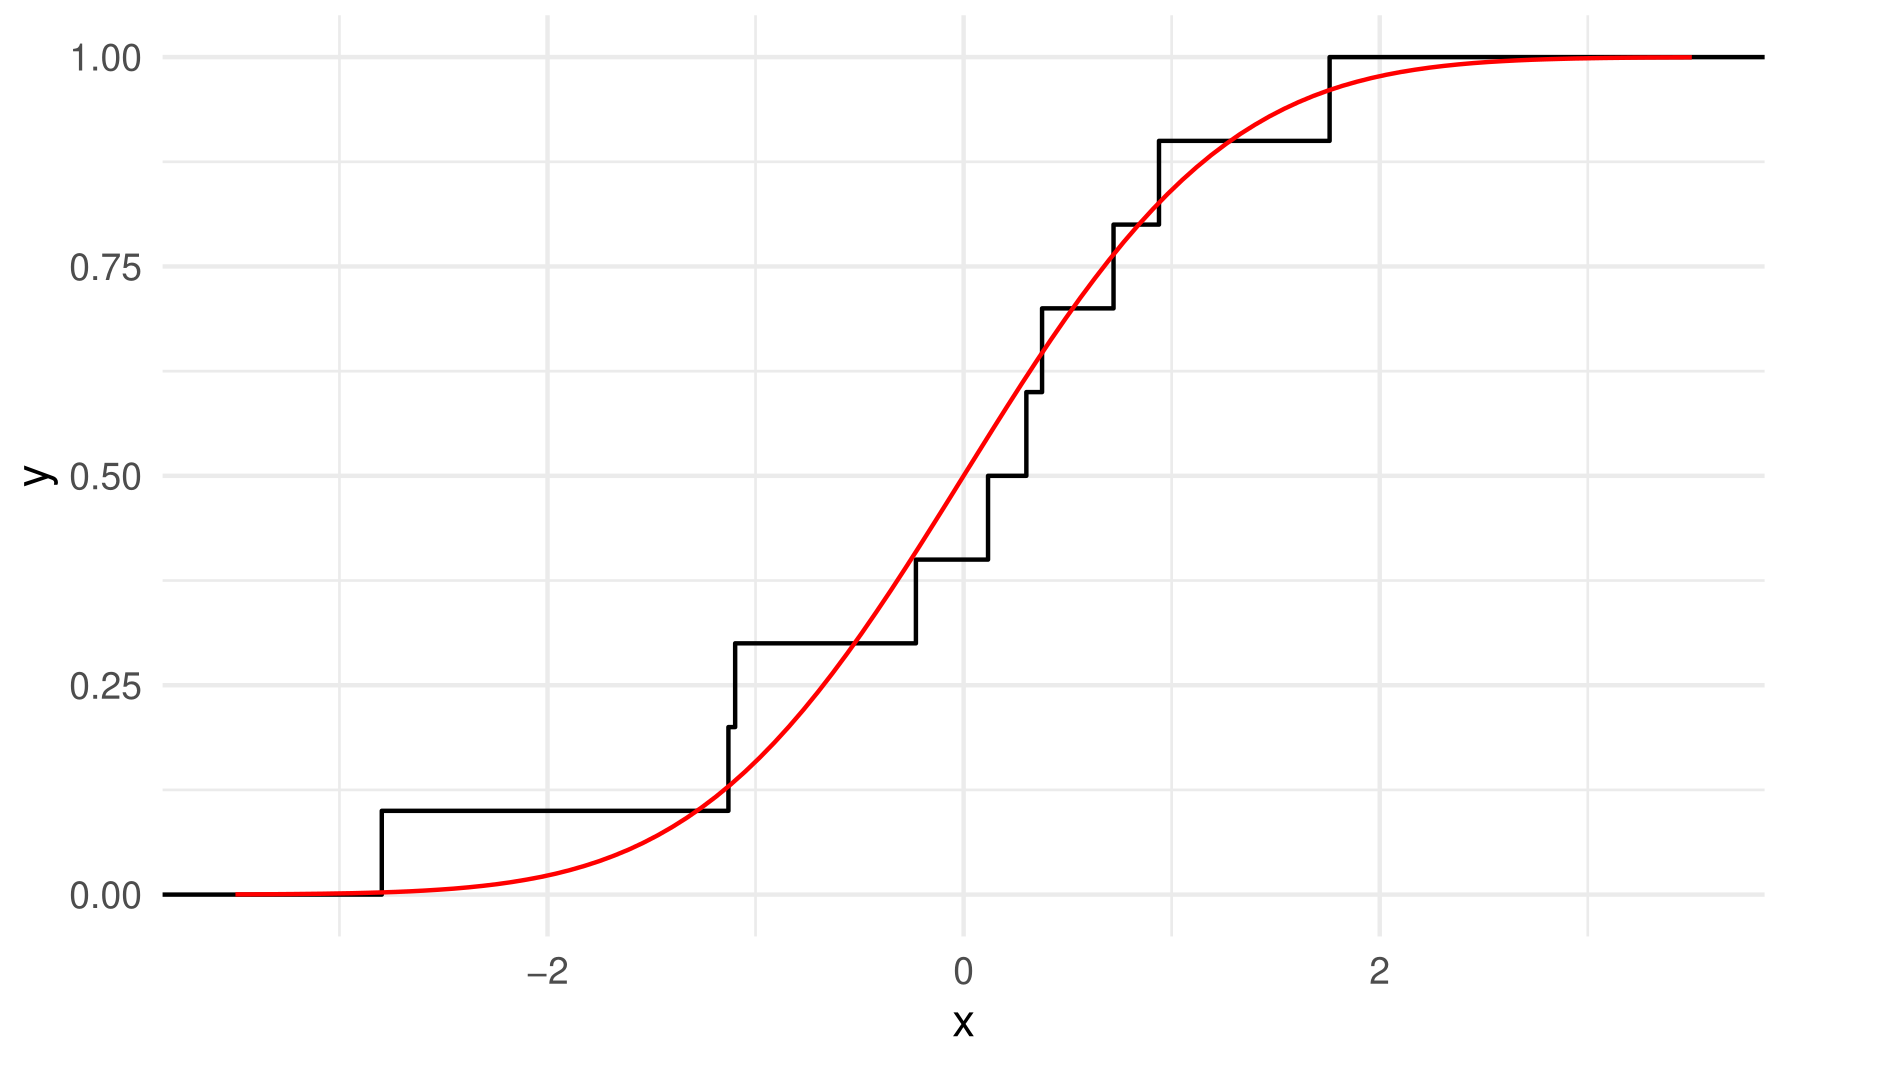
\includegraphics[width=0.8\textwidth]{./img/fms_cha2_ecdf.png}
    \caption{}
    \label{fig:ecdf}
\end{figure}

In \autoref{fig:ecdf}, the black curve represents the empirical cumulative distribution function (ECDF) based on 10 observations drawn from a standard normal distribution. The ECDF is a step function that increases by increments of \(1/10\) at each observed data point, taking the value \(0\) for sufficiently small arguments and \(1\) for sufficiently large ones. The locations of the jumps correspond to the unordered sample values, while their heights reflect the sample size. Since the data are drawn from a continuous distribution, ties occur with probability zero. The empirical distribution (black) roughly follows the true standard normal cumulative distribution function (red), illustrating how empirical proportions approximate theoretical probabilities in accordance with the law of large numbers.

\begin{note}[]
    From the ecdf we can recover the data points \(x_1, \dots , x_{n}\) up to their order, i.e., we can recover the order statistics.
\end{note}

Here is the plot for a normal sample of size \(n = 500\).
\begin{minted}{R}
   set.seed(2020) 
   ggplot(data.fram(x = rnorm(500)), aes(x)) +
    stat_ecdf(geom = "step") + 
    geom_funtion(data = data.frame(x = c(-3.5, 3.5)),
        fun = pnorm, colour = "red")
\end{minted}

\begin{figure}[htpb]
    \centering
    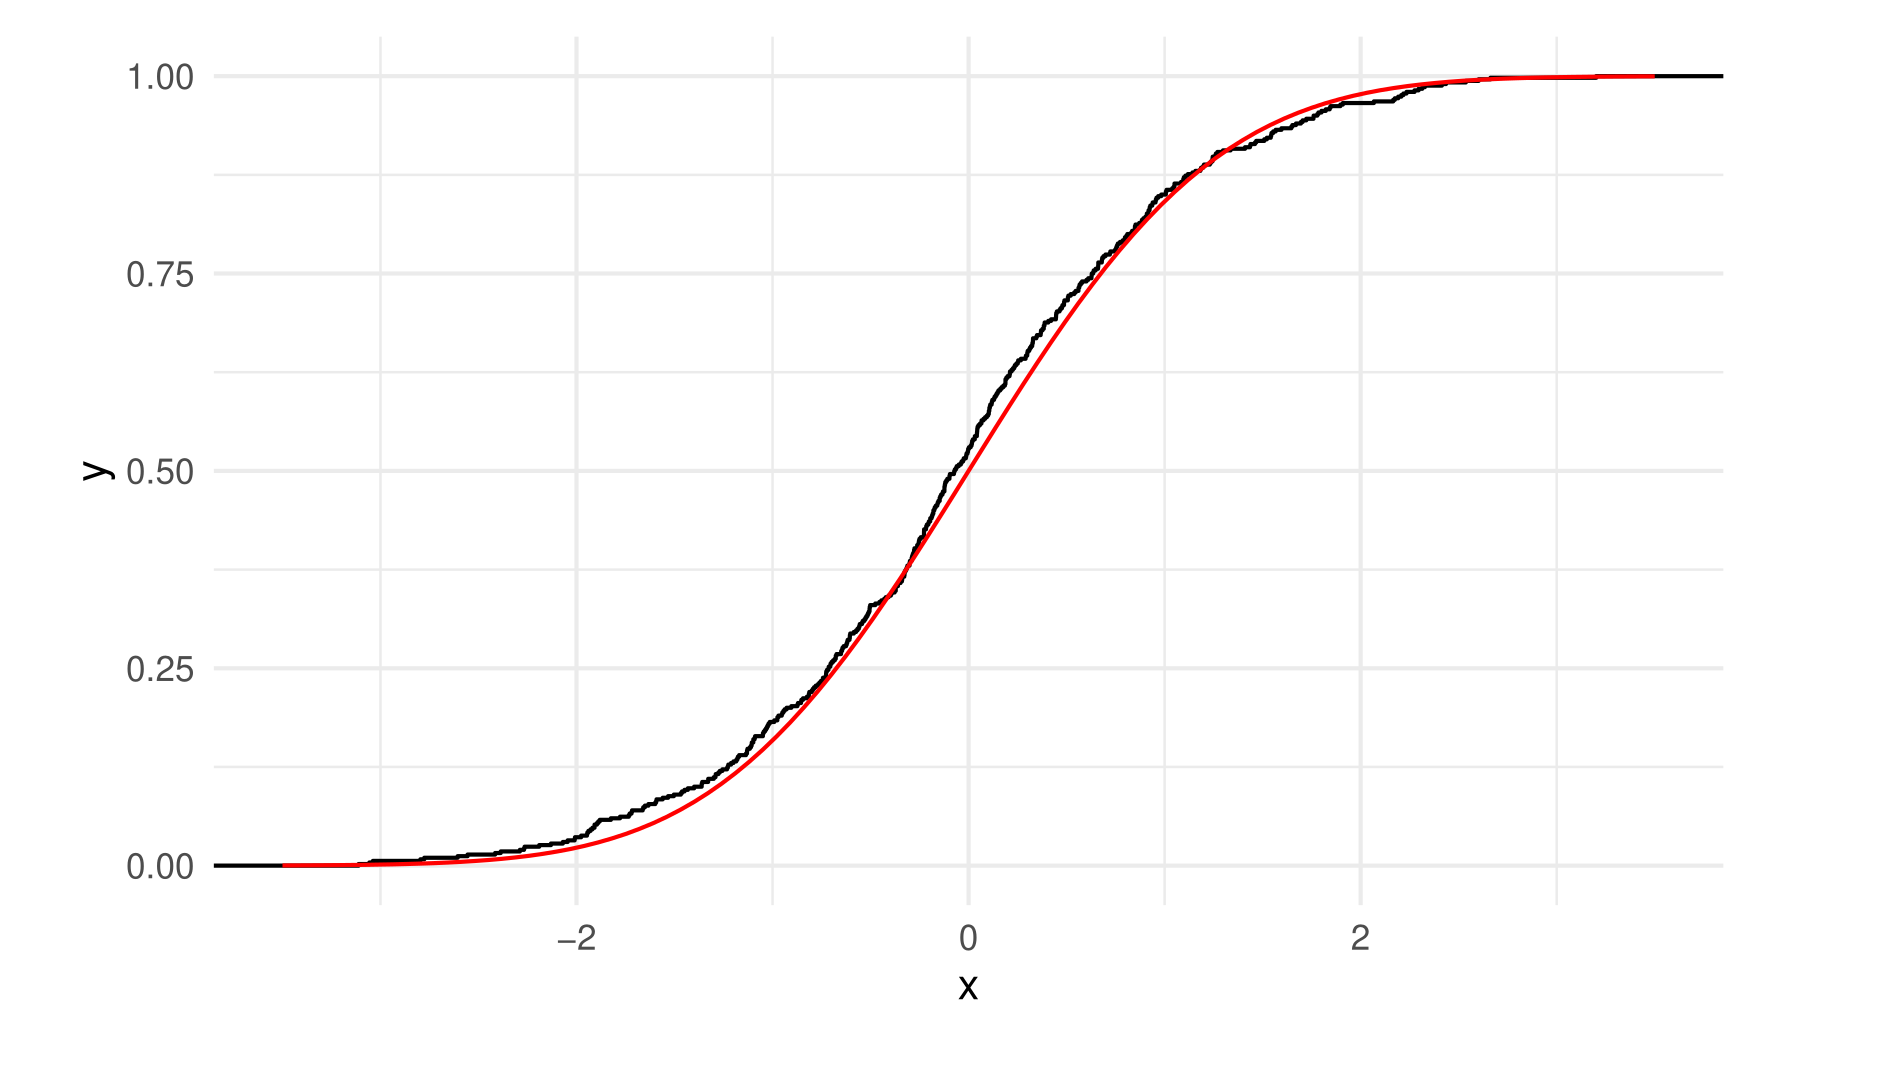
\includegraphics[width=0.8\textwidth]{./img/fms_cha2_ecdf500}
    \caption{}
    \label{fig:ecdf500}
\end{figure}

For a larger sample size, the empirical cumulative distribution function (ECDF) becomes smoother, since the jump size decreases as the number of observations increases. Although the ECDF may locally deviate from the true distribution function, it follows it closely overall. As the number of i.i.d. observations grows, the ECDF converges to the underlying distribution function. This shows that the ECDF is a consistent estimator of the true distribution function and highlights its connection to fundamental results such as the law of large numbers and the central limit theorem.

\subsection{Glivenko-Cantelli Theorem}%
\label{sub:Glivenko-Cantelli Theorem}


Let \(X_1,X_2,\dots \) be real valued r.v. (random variables) that are i.i.d. with cdf \(F\).

For any fixed \(t \in \R\),  the probability \(F(t)\) can be interpreted as the success probability of the indicator r.v. \(\mathbf{1}_{\{X_i \le t\}}\), which is then clearly a Bernoulli r.v. with parameter \(F(t)\), so we have
\[
    \mathsf{P}(X_{i}\le t) = F(t) \quad \text{and}\quad \bs{1}_{\{X_{i}\le t\}}\sim \text{Bernoulli}(F(t)),
\]
so \[
    \mathsf{E}[\bs{1}_{\{X_{i}\le t\}}] = F(t),
    \quad 
    \mathsf{Var}[\bs{1}_{\{X_{i}\le t\}}] = F(t)(1-F(t)).
\]

The empirical distribution function evaluated at \(t\) can therefore be interpreted as the average of these indicator variables, linking it directly to fundamental results such as the law of large numbers.

\myparagraph{Strong law of large numbers:}%

\label{par:Strong law of large numbers:}
Since these indicators have finite expectation, the Strong Law of Large Numbers applies.
\begin{align*}
    &\hat{F}_{n}(t) \equiv \hat{F}_{n}(t;X_1,\dots ,X_{n}) \overset{a.s.}{\longrightarrow}F(t), \\
    &\text{i.e.,}\quad \mathsf{P}\left( \lim\limits_{n \to \infty} \hat{F}_{n}(t) = F(t) \right) =1.
\end{align*}

Thus, for each fixed \(t\), the value of the empirical distribution function converges almost surely to the corresponding value of the true distribution function. In particular, as the sample size increases, the empirical proportion of observations less than or equal to \(t\) converges with probability one to \(F(t)\).

\myparagraph{Central limit theorem:}%
\label{par:Central limit theorem:}

For a fixed 
\(t \in \R\)
, the Central Limit Theorem describes the fluctuation (the \textbf{error} ) of the empirical distribution function around the true distribution function. After scaling by 
\(\sqrt{n} \)
, the estimation error 
\(\hat{F}_{n}(t) - F(t)\)
converges in distribution to a centered normal distribution with variance 
\(F(t)(1-F(t)\)
. 
This variance is inherited from the underlying Bernoulli indicator variables and quantifies the typical size of the estimation error.

\[
    \sqrt{n} (\hat{F}_{n}(t) - F(t)) \overset{d}{\longrightarrow} \cc{N}\left(0,F(t)(1-F(t))\right).
\]
Thus, for large \(n\), the estimation error at a fixed point \(t\) behaves approximately like a centered normal random variable with variance \(F(t)(1-F(t))\). This variance is maximized when \(F(t)=1/2\) and decreases as \(F(t)\) approaches \(0\) or \(1\), indicating smaller fluctuations in the tails of the distribution, and bigger on the middle of the distribution. 

\begin{note}[]
    Convergence in distribution: \(Y_{n} \overset{d}{\longrightarrow}Y\) if and only if \(F_{Y_{n}}(y) \underset{n \to \infty}{\longrightarrow}F_{Y}(y)\) at all points \(y \in \R\) at which \(F_{Y}\) is continuous.
\end{note}

The Strong Law of Large Numbers (SLLN) ensures that, for each fixed \(t \in \mathbb{R}\),
\[
\hat F_n(t) \equiv \frac{1}{n} \sum_{i=1}^n \mathbf{1}_{\{X_i \le t\}} \;\;\overset{\text{a.s.}}{\longrightarrow}\;\; F(t).
\]
In other words, the empirical CDF (black curve) converges almost surely to the true CDF (red curve) at any individual point.  

However, this is \emph{pointwise convergence}: it applies separately for each \(t\), and does not automatically guarantee that the empirical CDF approximates the true CDF uniformly over all points. In particular, some regions of the distribution—often the tails—may require much larger sample sizes for the approximation to be accurate.  

This motivates \emph{plug-in estimation}. If we want to estimate a functional of the underlying distribution (e.g., the median), we can compute it using the empirical CDF:
\[
\text{Estimate of } \theta(F) \;\;=\;\; \theta(\hat F_n),
\]
where \(\theta\) is any functional (mean, median, quantile, etc.). The idea is that the empirical CDF provides a good pointwise approximation to the true distribution, which can then be used to estimate various characteristics of the underlying data-generating process.

While the SLLN and CLT provide guarantees at individual points, they do not automatically control the empirical CDF as a whole. Since there are uncountably many points \(t \in \mathbb{R}\), the number of samples required for a good approximation may vary across the domain. For points in the tails (\(F(t)\) very small or very large), much larger sample sizes are needed for the CLT to provide an accurate normal approximation.

This motivates the question: can classical limit theorems (SLLN) be strengthened to show that the empirical CDF estimates the entire true distribution function simultaneously? Yes, and this is the content of the \emph{Glivenko–Cantelli theorem}. It provides a uniform convergence guarantee, ensuring that the black ECDF approaches the red true CDF across the whole domain.

\begin{theo}[Glivenko-Cantelli]
\label{theo:Glivenko-Cantelli}
    If \(X_1,X_2, \dots \) are i.i.d. r.v. with cdf F, 
then the empirical CDF
\[
\hat{F}_n(t) := \frac{1}{n} \sum_{i=1}^{n} \mathbf{1}_{\{X_i \le t\}}
\]
satisfies
    \[
        \|\hat{F}_{n}-F\|_{\infty} := \sup\limits_{t \in \R} \mid \hat{F}_{n}(t;X_1,\dots ,X_{n}) - F(t)\mid \overset{a.s.}{\longrightarrow}0.
    \]
\end{theo}

The Glivenko-Cantelli theorem strengthens the Strong Law of Large Numbers to uniform convergence over all \(t \in \mathbb{R}\).  
It also addresses the global accuracy of the empirical CDF. Instead of evaluating convergence at a single point \(t\), it considers the maximal deviation across all \(t \in \mathbb{R}\).  

By taking the supremo of the norm, we measure the worst-case difference between \(\hat{F}_n(t)\) and \(F(t)\). The theorem guarantees that this maximal deviation converges to zero almost surely.  
Intuitively, the empirical CDF (black curve) approximates the true CDF (red curve) uniformly across the entire real line as \(n\) grows.  

Glivenko-Cantelli can be seen as a uniform Law of Large Numbers for the indicator functions \(\mathbf{1}_{\{X_i \le t\}}\), and Donsker's theorem is the corresponding functional analog of the Central Limit Theorem.  

\begin{remark}[]
    \leavevmode
    \begin{itemize}
    \item Glivenko-Cantelli is a LLN for \(\hat{F}_{n}\) as element of a function space. The ``functional generalization'' of the CLT statement is known as Donsker's theorem.
    \item Empirical process theory generalizes these results to more general settings. For example, Glivenko-Cantelli results of the form \[
            \sup\limits_{f \in \cc{F}} \left|\frac{1}{n} \sum\limits_{i=1}^{n} f(X_{i}) - \mathsf{E}[f(X_{i})] \right| \overset{a.s.}{\longrightarrow}0.
    \]
    \end{itemize}
\end{remark}

\begin{proof}[\autoref{theo:Glivenko-Cantelli}]
    We first prove the theorem in the special case where \(X_1,X_2,\dots \) are i.i.d Unif(0,1), so \(F(t) = t\) for \(t \in [0,1]\).    

    \textbf{Idea:} Partition domain [0,1] \emph{finite} number of blocks and use monotonicity of cdf to control behaviour in each block.

The main difficulty in the theorem is that $\hat F_n(t)$ defines a random variable for 
each $t \in \mathbb{R}$, so we are dealing with an uncountable collection of random variables. 
However, the key property we exploit is \textbf{monotonicity}:
\begin{itemize}
    \item The true CDF $F$ is strictly increasing on $[0,1]$.
    \item The empirical CDF $\hat F_n$ is a non-decreasing step function.
\end{itemize}
This monotonicity allows us to control the sup-norm deviation of $\hat F_n$ from $F$ over 
an entire interval by examining finitely many points.

For any \(M \in \mathbb{N}\), we partition \([0,1]\) into \(M\) subintervals of equal length:
\[
I_j := \left[ \frac{j-1}{M}, \frac{j}{M} \right], \quad j=1,\dots,M.
\]

Within each interval, monotonicity implies that the maximum deviation of $\hat F_n(t)$ 
from $F(t)$ occurs at the endpoints. 
Then, by the monotonicity of \(\hat{F}_{n}\) and \(F\),
    \begin{align*}
        \|\hat{F}_{n}-F\|_{\infty} &= 
        \max\limits_{1\le j\le M} \sup\limits_{t \in \left[ \frac{j-1}{M},\frac{j}{M} \right] } \mid \hat{F}_{n}-F(t)\mid \\
                                   &=\max\limits_{1\le j\le M} \sup\limits_{t \in \left[ \frac{j-1}{M},\frac{j}{M} \right] } \max\{ \hat{F}_{n}-F(t), F(t) - \hat{F}_{n}(t)\} \\
                                   & \overset{\hat{F}_{n}\uparrow,F\uparrow}{\le } \max\limits_{1\le j\le M} \max \left\{ \hat{F}_{n}\left( \frac{j}{M} \right) -F \left( \frac{j-1}{M} \right) , F\left( \frac{j}{M}  \right) - \hat{F}_{n} \left( \frac{j-1}{M} \right)  \right\} 
                                   \\&= \max\limits_{1\le j\le M} \max \left\{ \hat{F}_{n}\left( \frac{j}{M} \right) -\frac{j-1}{M} ,\frac{j}{M}  - \hat{F}_{n} \left( \frac{j-1}{M} \right)  \right\} 
                                   \\&= \max\limits_{1\le j\le M} \max \left\{ \hat{F}_{n}\left( \frac{j}{M} \right) -\frac{j}{M} ,\frac{j-1}{M}  - \hat{F}_{n} \left( \frac{j-1}{M} \right)  \right\} + \frac{1}{M}.
    \end{align*}

Since there are only finitely many endpoints, we can apply the Strong Law of Large Numbers at each endpoint.
    For all \(j=1,\dots ,M\), \[
        \hat{F}_{n}\left( \frac{j}{M} \right) \overset{a.s.}{\longrightarrow} \frac{j}{M}.
    \]
    Hence, with probability one, \[
        \lim\limits_{n \to \infty} \max\limits_{1\le j\le M} \max \left\{ \hat{F}_{n}\left( \frac{j}{M} \right) -\frac{j}{M}, \frac{j-1}{M}-\hat{F}_{n}\left( \frac{j-1}{M} \right)  \right\} = 0.
    \]
    On the same event of probability one,
    \[
        \lim\limits_{n \to \infty} \sup \| \hat{F}_{n}-F\|_{\infty}\le \frac{1}{M}.
    \]
    Since \(M\) was arbitrary, we conclude that \[
        \| \hat{F}_{n}-F\|_{\infty} \overset{a.s.}{\longrightarrow}0.
    \]
    We will finish the proof for general r.v. at the end of the next section ...
\end{proof}


\begin{figure}[h!]
    \centering
    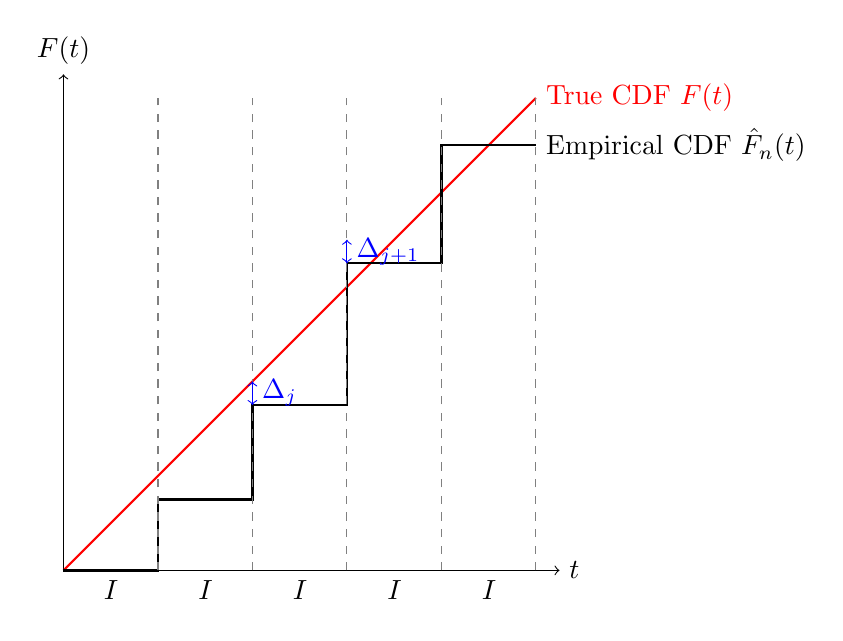
\begin{tikzpicture}[scale=6]
        % axes
        \draw[->] (0,0) -- (1.05,0) node[right] {$t$};
        \draw[->] (0,0) -- (0,1.05) node[above] {$F(t)$};

        % true CDF (red)
        \draw[thick,red] (0,0) -- (1,1) node[right] {True CDF $F(t)$};

        % empirical CDF (black, step function)
        \draw[thick,black] (0,0) -- (0.2,0) -- (0.2,0.15) -- (0.4,0.15) -- (0.4,0.35)
                            -- (0.6,0.35) -- (0.6,0.65) -- (0.8,0.65) -- (0.8,0.9) -- (1,0.9) 
                            node[right] {Empirical CDF $\hat F_n(t)$};

        % partition lines
        \foreach \x in {0.2,0.4,0.6,0.8,1.0} {
            \draw[dashed,gray] (\x,0) -- (\x,1);
        }

        % labels for partitions
        \foreach \x in {0.1,0.3,0.5,0.7,0.9} {
            \node[below] at (\x,0) {$I_{\pgfmathtruncatemacro{\j}{int(\x*5+0.5)}}$};
        }

        % max deviation arrows (optional)
        \draw[<->,blue] (0.4,0.35) -- (0.4,0.4) node[midway,right] {$\Delta_j$};
        \draw[<->,blue] (0.6,0.65) -- (0.6,0.7) node[midway,right] {$\Delta_{j+1}$};
    \end{tikzpicture}
    \caption{Illustration of the partition argument in the proof of the Glivenko-Cantelli theorem. The black curve is the empirical CDF, the red curve is the true CDF, and dashed gray lines indicate the partition intervals. The blue arrows show maximal deviation in each interval.}
    \label{fig:GC-partition}
\end{figure}

\begin{remark}[]
\leavevmode    
\begin{itemize}
    \item This argument reduces the problem from an uncountable collection of random variables 
    to finitely many points using the monotonicity of the CDF and empirical CDF.
    \item The extension to a general distribution $F$ is straightforward via the probability 
    integral transform: if $X_i \sim F$, then $F(X_i) \sim \mathrm{Unif}(0,1)$.
\end{itemize}
\end{remark}

\subsection{Quantile Function and Uniform Representation}%
\label{sub:Quantile Function and Uniform Representation}

Having established the Glivenko-Cantelli theorem for \(\mathrm{Unif}(0,1)\) random variables, 
we can now discuss how to extend this result to general distributions and motivate the 
\emph{plug-in principle} for estimation.

\medskip

For uniform random variables, the proof is convenient because the distribution function 
is explicit: \(F(t) = t\) on \([0,1]\). This allows us to evaluate the empirical CDF 
\(\hat F_n\) at specific grid points and directly control its deviation from \(F\).

\medskip

To generalize, consider a random variable \(X\) with cumulative distribution function \(F\). 
Recall that \(F\) is non-decreasing:
\[
F(t) = \Pr[X \le t], \quad t \in \mathbb{R}.
\]
If \(F\) is strictly increasing, it admits a well-defined inverse. Even if \(F\) is flat 
over some interval \([a,b]\), meaning \(F(a) = F(b)\), this simply indicates that \(X\) 
does not take values in \([a,b]\) with positive probability. 

\medskip

This motivates the definition of the \emph{generalized inverse} (or \emph{quantile function}).

The \textbf{quantile function} of a cdf \(F\) is the left-continuous function
\[
F^{-1}(q) = \inf \{ x \in \mathbb{R} : F(x) \ge q \}, \quad q \in (0,1).
\]

This definition assigns to each \(q \in (0,1)\) the smallest value \(x\) such that 
the distribution function reaches or exceeds \(q\). 

The quantile function allows us to map uniform random variables to a general distribution 
and thereby extend results proven for the uniform case to arbitrary distributions. 
This forms the basis of the plug-in principle: given an estimator \(\hat F_n\) of \(F\), 
we can estimate functionals of \(F\) by \(\phi(\hat F_n)\).

\medskip
Recall that \(F(t)\) is right-continuous.

\begin{remark}[]
\leavevmode    
\begin{itemize}
    \item If \(F\) is strictly increasing, the quantile function coincides with the usual inverse.
    \item In general, \(F^{-1}\) is a well-defined function for any distribution function \(F\).
    \item By the right-continuity of \(F\) (a property of all distribution functions), 
    the quantile function \(F^{-1}\) is \emph{left-continuous}.
\end{itemize}
\end{remark}

\textit{Question:} What is the quantile function of this cdf?
\begin{figure}[htpb]
    \centering
    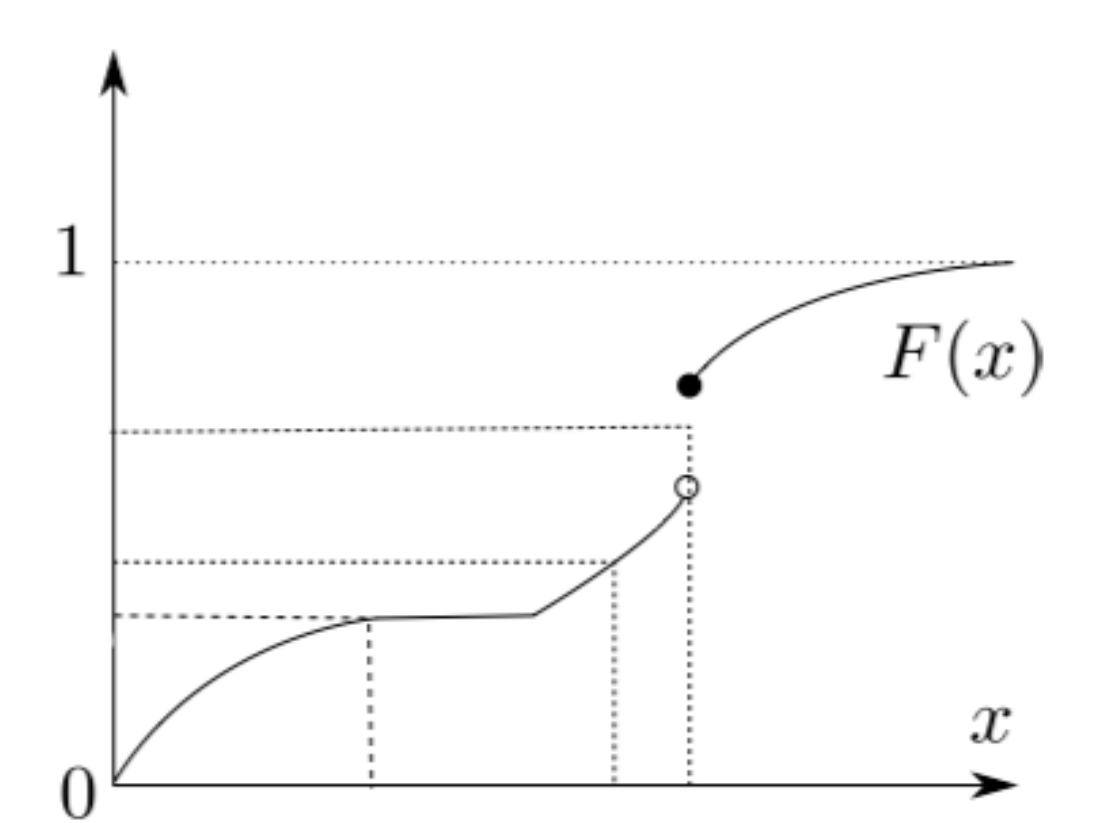
\includegraphics[width=0.5\textwidth]{./img/cha2_question}
    \caption{}
    \label{fig:cha2_question}
\end{figure}    

Suppose we are given a cdf \(F\) as a graph. 
The graph may have the following features:  
\begin{itemize}
    \item
an initial flat segment at \(0\),  
\item  a strictly increasing portion,  
\item  a flat interval,  
\item  jumps (discontinuities) due to the right-continuity of \(F\),  
\item  and it eventually converges to \(1\).  
\end{itemize}

The quantile function \(F^{-1}\) can be interpreted as a “generalized inverse” of this graph. Graphically:

\begin{itemize}
    \item A strictly increasing segment of \(F\) becomes an increasing segment of \(F^{-1}\).  
    \item A flat segment of \(F\) (where \(F\) does not increase) becomes a \emph{jump} in \(F^{-1}\) — we take the lower endpoint of the interval.  
    \item A jump in \(F\) (where \(F\) jumps upward due to right-continuity) becomes a flat segment in \(F^{-1}\).  
\end{itemize}

\medskip

In other words, to obtain the graph of the quantile function, one can “reflect” \(F\) across the diagonal \(y=x\), and then interpret flat segments and jumps according to the rules above. This construction ensures that \(F^{-1}\) is left-continuous and correctly represents the distribution of quantiles.  

\medskip

\textbf{Exercise:} Draw \(F\) with an increasing segment, a flat interval, and a jump, and then sketch the corresponding \(F^{-1}\) to see these transformations in action.

\myparagraph{Uniform Representation}%
\label{par:Uniform Representation}
\begin{lemma}
    \label{lemma:uni_repre}
    If \(U \sim Unif(0,1)\), then \(X := F^{-1}(U)\) has cdf \(F\).
\end{lemma}

Quantile functions provide a powerful tool for generating random variables with a desired distribution. Specifically, if we want a random variable \(X\) with cdf \(F\), we can construct it by transforming a uniform random variable \(U \sim \mathrm{Unif}(0,1)\) through the quantile function:
\[
    X = F^{-1}(U).
\]

This works because the quantile function maps the uniform probability space \([0,1]\) into the distribution defined by \(F\). For example, if \(F\) is the cdf of a standard normal distribution, then \(F^{-1}(U)\) produces a standard normal random variable. 

\begin{figure}[h!]
\centering
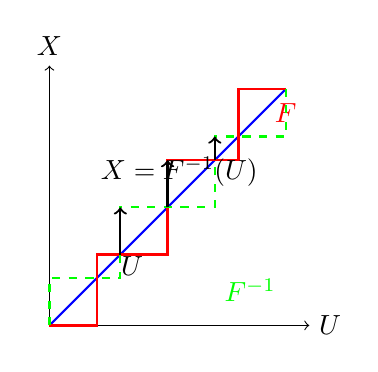
\begin{tikzpicture}[scale=3]

% Axes
\draw[->] (0,0) -- (1.1,0) node[right] {$U$};
\draw[->] (0,0) -- (0,1.1) node[above] {$X$};

% Uniform line (horizontal)
\draw[blue, thick] (0,0) -- (1,1); % identity line for reference

% Example CDF F
\draw[red, thick] (0,0) -- (0.2,0) -- (0.2,0.3) -- (0.5,0.3) -- (0.5,0.7) -- (0.8,0.7) -- (0.8,1) -- (1,1);
\node[red] at (1,0.9) {$F$};

% Quantile function F^{-1}
\draw[green, thick, dashed] (0,0) -- (0,0.2) -- (0.3,0.2) -- (0.3,0.5) -- (0.7,0.5) -- (0.7,0.8) -- (1,0.8) -- (1,1);
\node[green] at (0.85,0.15) {$F^{-1}$};

% Arrows showing mapping
\draw[->, thick] (0.3,0.3) -- (0.3,0.5);
\draw[->, thick] (0.7,0.7) -- (0.7,0.8);
\draw[->, thick] (0.5,0.5) -- (0.5,0.7);

% Labels
\node at (0.35,0.25) {$U$};
\node at (0.55,0.65) {$X = F^{-1}(U)$};

\end{tikzpicture}
\caption{Graphical interpretation of the uniform representation: mapping a uniform random variable $U$ to a random variable $X$ with CDF $F$ using the quantile function $F^{-1}$.}
\end{figure}

This construction is the basis of one of the simplest and most fundamental methods for simulating random variables on a computer: start with a uniform random number generator, then transform the output via the quantile function of the desired distribution. 

While this is conceptually straightforward, in practice there are often more efficient simulation methods implemented in statistical software packages such as R. Nevertheless, the uniform representation is extremely useful for both theoretical and practical purposes, as it allows us to write any random variable of interest explicitly as a function of a uniform random variable. Such representations are widely used in probability theory, simulation, and Monte Carlo methods.

\begin{proof}[\autoref{lemma:uni_repre}]
    For any \(u \in (0,1)\) and \(x \in \R\),
the quantile function $F^{-1}$ satisfies
     \[
        F^{-1}(u) \le x \iff u \le F(x).
    \]
   \begin{description}
       \item[(\(\Longleftarrow\))] : Follows from the definition of \(F^{-1}(u)\) as an infimum.
       \item[(\(\Longrightarrow\))] : Follows by observing that \[
           F^{-1}(u) \le x \implies F(x + \eps) \ge  u \quad \forall \eps >0 
       \]
        taking \(\eps \to 0\) and using the right-continuity of $F$ gives $F(x) \ge u$.
    \end{description}
 Since $U \sim \text{Unif}(0,1)$, using \autoref{theo:Glivenko-Cantelli}, we obtain that for all \(x \in \R\),\[
       \mathsf{P}(X\le x) = \mathsf{P}(F^{-1}(U)\le x) = \mathsf{P}(U\le F(x)) = F(x).
   \]
\end{proof}

\begin{proof}[\autoref{theo:Glivenko-Cantelli} Glivenko-Cantelli for general r.v.]
    Let \(U_1,U_2,\dots \) be i.i.d Unif(0,1) with cdf \(G(t)=t,t\in[0,1]\).


By the uniform (quantile) representation, the sequence
\[
X_i := F^{-1}(U_i), \qquad i=1,2,\dots,
\]
is i.i.d.\ with cdf \(F\). In particular, the joint distribution of
\((X_1,X_2,\dots)\) coincides with that of
\((F^{-1}(U_1),F^{-1}(U_2),\dots)\).
%    Original sequence \((X_{i})^{\infty}_{i=1}\) has same joint distribution as \((F^{-1}(U_{i}))^{\infty}_{i=1}\).

    Let \(\hat{G }_{n}\) be the ecdf of \(U_1,\dots ,U_{n}\). Then for every \(n\),
    \begin{align*}
        \hat{F}_{n}(t) = \frac{1}{n}\sum\limits_{i=1}^{n} \bs{1}_{\{X_{i}\le t\}} 
        &\underset{d}{=} \frac{1}{n} \sum\limits_{i=1}^{n} \bs{1}_{\{F^{-1}(U_{i})\le t\}}\\
        &= \frac{1}{n}\sum\limits_{i=1}^{n} \bs{1}_{\{U_{i}\le F(t)\}}= \hat{G }_{n}(F(t)), 
    \end{align*}
    where \autoref{lemma:uni_repre} was used in the second last equality. 

    Noting that \(G(F(t)) = F(t)\), we conclude that 
\[
\|\hat F_n - F\|_\infty \overset{d}{=} \| \hat{G }_{n} \circ F - G \circ F\|_{\infty}
= \sup_{t \in \mathbb{R}}
\bigl|\hat G_n(F(t)) - G(F(t))\bigr|.
\]
Since \(F(t) \in [0,1]\) for all \(t\), we obtain the bound
\[
\|\hat F_n - F\|_\infty
= \sup\limits_{t \in \R} \bigl| \hat{G }_{n}(F(t)) - G(F(t)) \bigr|
\le \sup_{t \in [0,1]} \bigl|\hat G_n(t) - G(t)\bigr|
= \|\hat G_n - G\|_\infty.
\]

By the Glivenko-Cantelli \autoref{theo:Glivenko-Cantelli} for the uniform distribution,
\[
\|\hat G_n - G\|_\infty \xrightarrow{\text{a.s.}} 0.
\]
Therefore,
\[
\|\hat F_n - F\|_\infty \xrightarrow{\text{a.s.}} 0,
\]
which proves the theorem for a general distribution function \(F\).
%    \[
%        \|\hat{F}_{n}-F\|_{\infty} \underset{d}{=} \| \hat{G }_{n} \circ - G \circ F \|_{\infty}\le \| \hat{G }_{n}-G\|_{\infty}.
%    \] 
%    The distributional equality holds jointly across all \(n\). Hence,\[
%        \|\hat{G}_{n}-G\|_{\infty} \overset{a.s.}{\longrightarrow} 0 \implies \| \hat{F}_{n}-F\|_{\infty}\overset{a.s.}{\longrightarrow}0.
%    \]
\end{proof}

\subsection{Plug-in Estimation}%
\label{sub:Plug-in Estimation}

The Glivenko--Cantelli theorem suggests replacing the unknown 
cdf \(F\) with the ecdf \(\hat F_n\) when
estimating a statistical parameter of the form \(\gamma(F)\), where
\(\gamma\) is a functional defined on distributions and
\(X_1, \dots, X_n\) are i.i.d.\ r.v. with distribution \(F\).

\begin{definition}
The \textbf{plug-in estimator} of the parameter \(\gamma(F)\) is defined as
\[
\hat{\gamma} := \gamma(\hat F_n).
\]
\end{definition}

\begin{note}
The functional \(\gamma\) must be well defined for discrete distributions,
since the empirical distribution function \(\hat F_n\) is discrete.
\end{note}

The principle of plug-in estimation is conceptually straightforward.
Rather than attempting to estimate \(\gamma(F)\) directly, we first estimate
the underlying distribution \(F\) using the empirical distribution
\(\hat F_n\). We then compute the parameter of interest by applying the same
functional \(\gamma\) to \(\hat F_n\).

This approach provides a general and intuitive framework for constructing
estimators. Many parameters of interest, such as moments or quantiles, can be
expressed as functionals of the distribution. Plug-in estimation therefore
offers a natural way to estimate such quantities by substituting the unknown
distribution with its empirical counterpart.

\begin{ex}
Consider the mean (expectation) functional
\[
\gamma(F) = \int x \, dF(x).
\]
The corresponding plug-in estimator is obtained by replacing \(F\) with the
empirical distribution function \(\hat F_n\):
\[
\gamma(\hat F_n)
= \int x \, d\hat F_n(x)
= \frac{1}{n} \sum_{i=1}^n X_i
=: \bar X_n,
\]
which is the sample mean.
\end{ex}

This example illustrates the plug-in principle in a particularly simple
setting. The population mean is a functional that integrates the identity
function with respect to the distribution \(F\). To estimate it, we apply the
same functional to the empirical distribution \(\hat F_n\).

Since \(\hat F_n\) is a discrete distribution that assigns probability
\(1/n\) to each observation \(X_1, \dots, X_n\), integration with respect to
\(\hat F_n\) reduces to taking the average of the observed data points. Thus,
the mean of the empirical distribution coincides with the usual sample mean.

Many other estimators can be interpreted in the same way. Sample moments,
variances, and correlations arise by applying the corresponding functionals to
the empirical distribution.

The main limitation of this approach is that the functional must be well
defined for discrete distributions. In particular, functionals involving
densities cannot be directly estimated via plug-in methods, since the
empirical distribution does not admit a density with respect to Lebesgue
measure.


\section{M-Estimators}
\label{sec:M-Estimators}

An estimator \(\hat\theta = \hat\theta(X_1, \dots, X_n)\) that maximizes a
criterion function of the form
\[
\theta \mapsto \frac{1}{n} \sum_{i=1}^n m_\theta(X_i),
\]
where \(m_\theta\) is a known real-valued function, is called an
\textbf{M-estimator} (maximum-likelihood type).

M-estimation is a general principle for constructing estimators based on
optimization. The parameter estimate \(\hat\theta\) is obtained by maximizing
(or minimizing) an empirical objective function, often interpreted as an
average (empirical) loss or criterion evaluated at the observed data.

This framework is broad and includes many classical estimators. For instance,
in parametric models such as the normal distribution with unknown mean and
variance, parameter values can be chosen by optimizing an appropriate
criterion function. In practice, such criteria are typically expressed as
averages of the form \(m_\theta(X_i)\), with one contribution from each data
point.


\begin{ex}
\leavevmode
\begin{itemize}
    \item For \(\theta \in \mathbb{R}\), let
    \[
    m_\theta(x) = - (x - \theta)^2.
    \]
    The resulting M-estimator \(\hat\theta\) is the sample mean \(\bar X_n\).
    Indeed, for any random variable \(X\) with distribution function \(F\)
    and finite variance, the expectation satisfies
    \[
    \mathsf{E}[X]
    = \arg\min_{\theta \in \mathbb{R}}
    \mathsf{E}_{X \sim F}\bigl[(X - \theta)^2\bigr].
    \]
    Replacing \(F\) by the empirical distribution \(\hat F_n\) yields
    \begin{align*}
        \bar X_n
        = \gamma(\hat F_n)
        &= \arg\min_{\theta \in \mathbb{R}}
        \mathsf{E}_{X \sim \hat F_n}\bigl[(X - \theta)^2\bigr] \\
        &= \arg\min_{\theta \in \mathbb{R}}
        \frac{1}{n} \sum_{i=1}^n (X_i - \theta)^2.
    \end{align*}

    \item Replacing the squared loss by the absolute loss,
    \(m_\theta(x) = -|x - \theta|\),
    yields the sample median as the corresponding M-estimator.

    \item The \textbf{Huber estimator} is the M-estimator defined by
    \[
    m_\theta(x) = -\rho_c(x - \theta),
    \]
    where
    \[
    \rho_c(x) =
    \begin{cases}
        x^2, & \text{if } |x| \le c, \\
        c(2|x| - c), & \text{if } |x| > c.
    \end{cases}
    \]
\end{itemize}
\end{ex}

\myparagraph{Connection to plug-in estimation}
\label{par:connection_plugin}

M-estimation can be viewed as an application of the plug-in principle.
A parameter is defined as the optimizer of a \emph{population} objective
function, typically an expected loss under the data-generating distribution.
The corresponding estimator is obtained by replacing this expectation with an
empirical average computed from the sample.

For instance, the population mean can be characterized as the minimizer of the
expected squared deviation. Replacing the expectation by an average over the
data leads to the empirical squared loss, whose minimizer is the sample mean.
Thus, the sample mean can be interpreted both as a plug-in estimator and as an
M-estimator.

More generally, whenever a parameter can be expressed as the minimizer (or
maximizer) of an expected loss function, replacing the expectation by an
empirical mean yields an estimator of M-estimation type. Absolute loss leads to
the sample median, while other loss functions give rise to robust estimators
such as the Huber estimator.

Throughout, it is important to distinguish between \emph{population}
quantities—defined in terms of the true data-generating distribution—and
\emph{sample} quantities, which are computed from the observed data.

\section{Method of Moments (MOM)}
\label{sec:mom}

Suppose we observe real-valued data from a parametric model
\[
X_1, \dots, X_n \overset{\text{i.i.d.}}{\sim} \mathsf{P}_\theta,
\quad \theta \in \Theta \subseteq \mathbb{R}^k.
\]
For \(j = 1, \dots, k\), define the \(j\)-th moment of the distribution as
\[
\mu_j(\theta) = \mathsf{E}_\theta[X_i^j].
\]
Whenever it exists, the \(j\)-th moment can be estimated empirically by
\[
\hat\mu_j = \frac{1}{n} \sum_{i=1}^n X_i^j.
\]

\begin{definition}
The \textbf{method of moments (MOM) estimator} \(\hat\theta\) is defined as a
solution to the system of equations
\[
\mu_j(\theta) = \hat\mu_j, \quad j = 1, \dots, k.
\]
\end{definition}

\emph{Subtleties:} A solution to this system need not exist, and if it exists,
it may not be unique.

The intuition behind the method of moments is simple. For each parameter value
\(\theta\), the model implies specific values for the moments
\(\mu_1(\theta), \dots, \mu_k(\theta)\). On the other hand, these moments can be
estimated directly from the data by taking empirical averages. The method of
moments chooses the parameter value \(\hat\theta\) for which the theoretical
moments of the model match the empirical moments computed from the sample.

In practice, this leads to a system of \(k\) equations in \(k\) unknowns. Whether
this system admits a solution, and whether that solution is unique, depends on
the specific model under consideration.


\begin{ex}[Negative binomial model]
    \label{ex:nbm}
Let \(\mathrm{NegBin}(k,\theta)\) denote the distribution of the number of
failures observed until the \(k\)-th success in independent Bernoulli trials
with success probability \(\theta\).

Suppose
\[
X_1, \dots, X_n \overset{\text{i.i.d.}}{\sim} \mathsf{P}_\theta
= \mathrm{NegBin}(k,\theta),
\]
where \(k \in \mathbb{N}\) is known and \(\theta \in (0,1)\) is unknown. The
probability mass function is given by
\[
\mathsf{P}_\theta(X_i = x)
= \binom{k + x - 1}{x} \theta^k (1 - \theta)^x,
\quad x = 0,1,2,\dots
\]

Since there is a single unknown parameter, we use the first moment. The
expectation of \(X_i\) is
\[
\mu_1(\theta) = \mathsf{E}_\theta[X_i]
= \frac{k(1 - \theta)}{\theta}.
\]
The corresponding method of moments equation is
\[
\frac{k(1 - \theta)}{\theta}
\overset{!}{=}
\hat\mu_1
= \bar X_n.
\]
Solving for \(\theta\) yields the MOM estimator
\[
\hat\theta
= \frac{k}{\bar X_n + k}
= \frac{nk}{\sum_{i=1}^n X_i + nk}.
\]

This estimator admits the interpretation
\[
\hat\theta
= \frac{\text{total number of successes}}
       {\text{total number of trials}},
\]
since across the \(n\) experiments exactly \(nk\) successes are observed and
\(\sum_{i=1}^n X_i\) failures occur in total.
\end{ex}


\begin{ex}[Gaussian model]
Suppose
\[
X_1, \dots, X_n \overset{\text{i.i.d.}}{\sim} \mathcal{N}(\mu, \sigma^2),
\]
where both the mean \(\mu \in \mathbb{R}\) and the variance
\(\sigma^2 \in (0,\infty)\) are unknown. The parameter is
\[
\theta = (\mu, \sigma^2) \in \Theta = \mathbb{R} \times (0,\infty).
\]
The density of the normal distribution is
\[
p_\theta(x)
= \frac{1}{\sqrt{2\pi\sigma^2}}
\exp\!\left\{
-\frac{1}{2\sigma^2}(x - \mu)^2
\right\},
\quad x \in \mathbb{R}.
\]

Since there are two unknown parameters, we use the first two moments. The
population moments are
\begin{align*}
\mu_1(\theta)
&= \mathsf{E}_\theta[X_1]
= \mu,
\\
\mu_2(\theta)
&= \mathsf{E}_\theta[X_1^2]
= \mathsf{Var}_\theta(X_1) + \bigl(\mathsf{E}_\theta[X_1]\bigr)^2
= \sigma^2 + \mu^2.
\end{align*}
The corresponding method of moments equations are
\begin{align*}
\mu &= \bar X_n, \\
\sigma^2 + \mu^2 &= \hat\mu_2,
\end{align*}
where
\[
\hat\mu_2 = \frac{1}{n} \sum_{i=1}^n X_i^2.
\]

Solving this system yields the MOM estimators
\begin{align*}
\hat\mu &= \bar X_n, \\
\hat\sigma^2
&= \hat\mu_2 - (\bar X_n)^2
= \frac{1}{n} \sum_{i=1}^n X_i^2
- \left( \frac{1}{n} \sum_{i=1}^n X_i \right)^2 \\
&= \frac{1}{n} \sum_{i=1}^n (X_i - \bar X_n)^2.
\end{align*}
which are actually the sample mean and the empirical variance.
\end{ex}



\begin{ex}[Pareto model]
    Suppose \(P_{\theta}\) has the density \[
        p_{\theta}(x) = \theta \cdot (1+x)^{-(1+\theta)}, \quad x>0,
    \]
    with unknown parameter \(\theta \subseteq  \Theta = (0,\infty)\).

    Density for \(\theta \in \{0.5,1,2,3\}\):
    \begin{figure}[htpb]
        \centering
        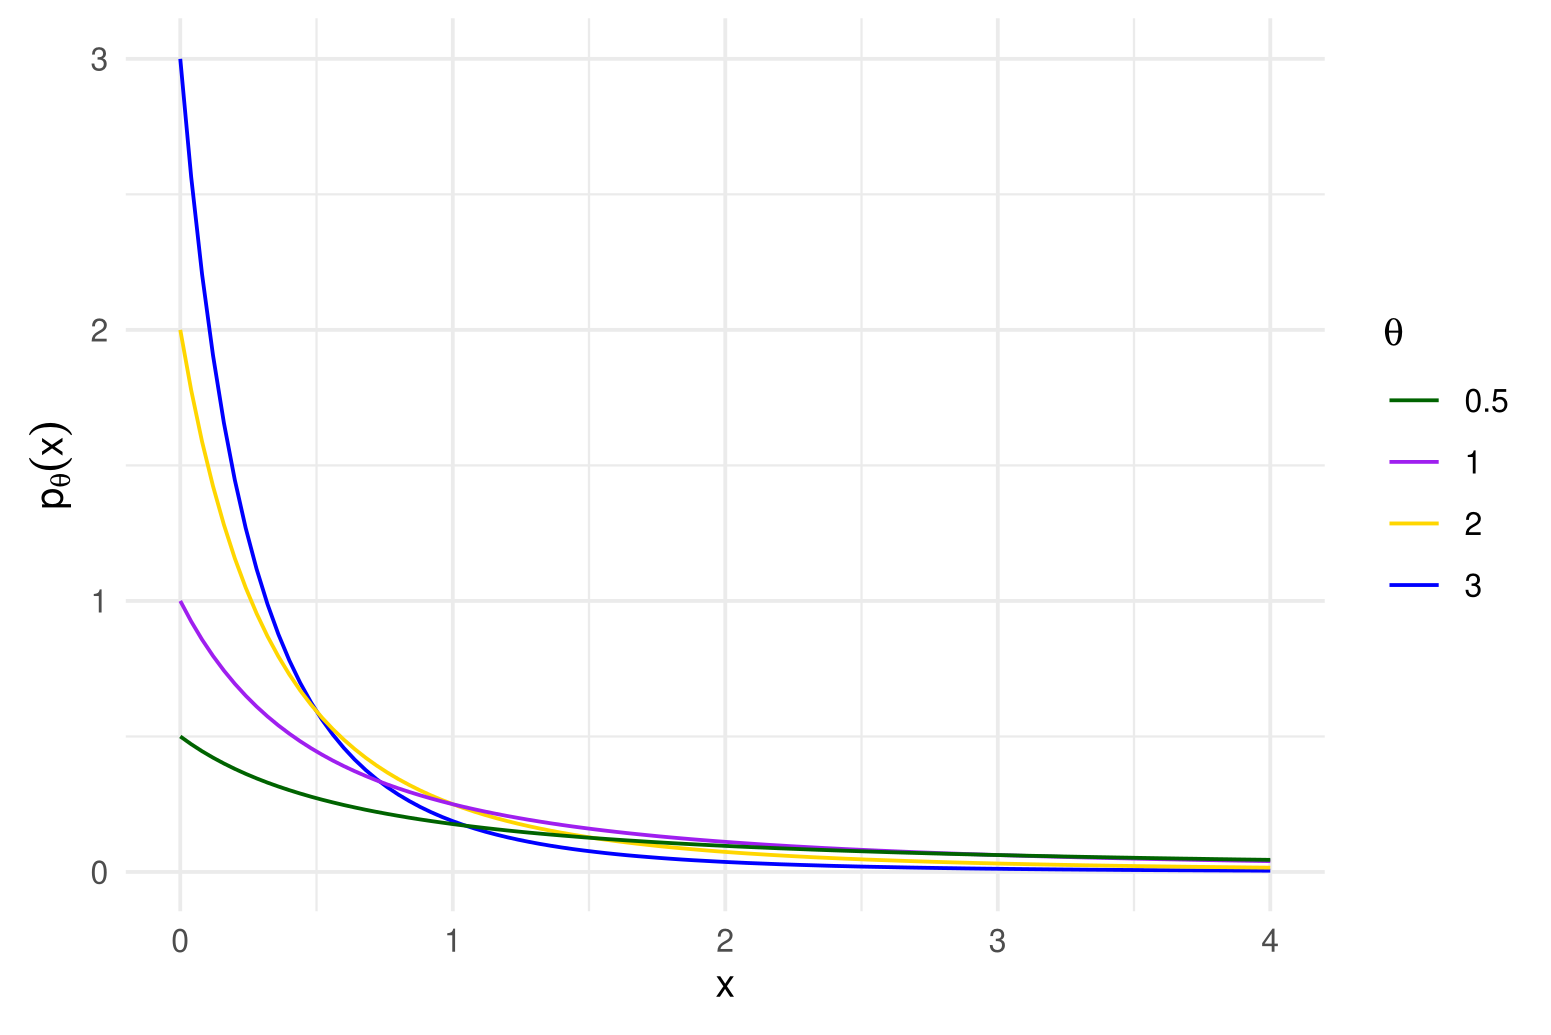
\includegraphics[width=0.8\textwidth]{./img/ch2_pareto}
        \caption{}
        \label{fig:pareto}
    \end{figure}

    First moment \(\mu_1(\theta) = \mathsf{E}_{\theta}[X_1]\) exists for which \(\theta\)?

    We have 
    \begin{align*}
        \mathsf{E}_{\theta}[X_1] &= \int_{0}^{\infty} x \theta \cdot (1+x)^{-(1+\theta)}dx\\
                                 &= x \cdot (1+x)^{-\theta}\mid^{\infty}_{0}+ \int_{0}^{\infty} (1+x)^{-\theta}dx
                              \\ &= \frac{1}{1-\theta}(1+x)^{-\theta+1}\mid^{\infty}_{0}\\
                                 &= \lim\limits_{a  \to \infty} \frac{1}{1-\theta}(1+a)^{-\theta+1}+\frac{1}{\theta-1},
    \end{align*}
    which is finite for \(\theta>1\).

    If \(\mu_1(\theta)\) exists, then the MOM is obtained by equating the sample mean \(\bar{X}_{n}\) with \(\mu_1(\theta)\) \[
        \mu_1(\theta) = \bar{X}_{n} = \frac{1}{\theta-1}.
    \]
    MOM estimator is \[
        \hat{\theta} = \frac{1+\bar{X}_{n}}{\bar{X}_{n}}.
    \]
    How do you think \(\hat{\theta}\) behaves if \(\mu_1(\theta)\) doesn't exists and we get a large sample (i.e., if \(n\) is large)?

    As sample size \(n\) increases, the MOM estimator is heavily influenced by extreme values and does not converge to the true \(\theta\). Instead, it tends to values around \(1\) or slightly above.
    \begin{remark}[]
    \leavevmode    
\begin{itemize}
    \item The estimator \(\hat{\theta}\) is always well-defined for any sample because \(\bar{X}_n>0\), even if the true mean does not exist (\(\theta \le 1\)).
    \item If \(\theta>1\), \(\hat{\theta}\) converges to the true parameter as \(n \to \infty\).
    \item If \(\theta \le 1\), the population mean does not exist. In this case, \(\hat{\theta}\) will still produce a value greater than 1, typically overestimating \(\theta\), because extreme values dominate the sample mean.
    \item This illustrates a general limitation of the method of moments: it assumes that the relevant population moments exist. Heavy-tailed distributions with non-existent moments can produce misleading estimates.
\end{itemize}
    \end{remark}
\end{ex}

\myparagraph{Comments on the Method of Moments (MOM)}%
\label{par:Comments on MOM}

\begin{itemize}
    \item By definition, the method of moments uses the first \(k\) population moments to estimate a \(k\)--dimensional parameter. Generally, higher-order moments (\(\mu_j\) with large \(j\)) are estimated less accurately by their sample counterparts \(\hat{\mu}_j\).
    
    \item For multivariate observations \(X_i = (X_{i1}, \dots, X_{id})\), one can consider expectations of each coordinate, their powers, and cross-products, e.g.,
    \[
        \mathsf{E}[X_{i1}],\ \mathsf{E}[X_{i2}],\ \mathsf{E}[X_{i1}^2],\ \mathsf{E}[X_{i1} X_{i2}],\ \mathsf{E}[X_{i2}^2], \dots
    \]
    \item More generally, one can use arbitrary functions \(h_1,\dots,h_k\) of the data to construct the equations
    \[
        \mathsf{E}_\theta[h_j(X_i)] = \frac{1}{n}\sum_{i=1}^{n} h_j(X_i), \quad j=1,\dots,k,
    \]
    potentially leading to improved estimators. The choice of the functions \(h_j\) is, however, not always obvious.
    
    \item In practice, powers of the observations are typically used because they often allow for closed-form calculations of expectations under the assumed model. This simplifies solving the moment equations.
    
    \item MOM can be extended to multivariate data by including powers and cross-products of the coordinates, forming monomials that define the estimating equations.
    
%    \item Historically, the method of moments was introduced by Pearson in 1894 to analyze Gaussian mixture models (e.g., crab populations) with up to five parameters. In that case, he solved a polynomial system of degree nine to obtain the MOM estimators.
    
    \item While maximum likelihood estimation often produces more efficient estimators and is preferred in many classical examples, the method of moments remains valuable. It can provide computationally simple and tractable estimators, especially in modern applications where closed-form or robust solutions are desired.
\end{itemize}

\begin{note}[]
Although sometimes considered a “classical” or “old-fashioned” method, MOM continues to be useful in practical and theoretical settings, albeit with some limitations in accuracy and uniqueness of solutions.
\end{note}

\section{Maximum Likelihood Estimation (MLE)}
\label{sec:MLE}

Consider a parametric statistical model for an observed random element
\[
    X \sim \mathsf{P}_{\theta}, \quad \theta \in \Theta \subseteq \mathbb{R}^{k}.
\]
The collection
\[
    \mathcal{P} = \{\mathsf{P}_{\theta} : \theta \in \Theta\}
\]
is referred to as a \emph{parametric model} with parameter space \(\Theta\).

We assume that the model is \emph{dominated}, meaning that there exists a
\(\sigma\)-finite measure \(\nu\) such that
\[
    \mathsf{P}_{\theta} \ll \nu \quad \text{for all } \theta \in \Theta.
\]
This assumption implies that every distribution in the model admits a
density with respect to \(\nu\), given by
\[
    p_{\theta}(x)
    = \frac{d \mathsf{P}_{\theta}}{d \nu}(x),
    \quad x \in \mathcal{X}.
\]

This framework encompasses both continuous and discrete models. For
instance, when \(\nu\) is Lebesgue measure, \(p_{\theta}\) is an ordinary
probability density function, while if \(\nu\) is counting measure,
\(p_{\theta}\) is a probability mass function. Throughout, we use
\(\mathsf{P}_{\theta}\) to denote the distribution of the data and
\(p_{\theta}\) to denote its corresponding density.

The maximum likelihood principle is one of the most widely used methods
for inference in parametric models. For simplicity of exposition, we
present the method for a single observation \(X\); the same framework
applies when \(X\) represents a sample, a vector, or a more general data
object.

\begin{definition}[Likelihood Function]
Let \(x \in \mathcal{X}\) denote an observed data point. The function
\[
    L_x(\theta) = p_\theta(x), \qquad \theta \in \Theta,
\]
is called the \textbf{likelihood function} of the model
\(\mathcal{P} = \{\mathsf{P}_\theta : \theta \in \Theta\}\) for the data \(x\).
\end{definition}

Recall that, for a fixed parameter value \(\theta\), the density
\(p_\theta(x)\) is a function of the data \(x\) and fully characterizes
the distribution \(\mathsf{P}_\theta\). Probabilities of events are
obtained by integrating this density with respect to the underlying
measure.

In likelihood-based inference, this perspective is reversed: the
observed data \(x\) is treated as fixed, and the density is viewed as a
function of the parameter \(\theta\). The resulting function
\(L_x(\theta)\) evaluates how compatible different parameter values are
with the observed data.

In discrete models, where \(p_\theta\) is a probability mass function,
\(L_x(\theta)\) coincides with the probability of observing the data
\(x\) under the distribution \(\mathsf{P}_\theta\). More generally, the
likelihood function provides a basis for comparing the relative
plausibility of different parameter values given the data.

\begin{definition}[Maximum Likelihood Estimation (MLE)]
The \textbf{maximum likelihood estimate (MLE)} of \(\theta\) based on observed
data \(x\) is defined as
\[
    \hat{\theta}(x)
    = \arg\max_{\theta \in \Theta} L_x(\theta),
\]
where \(L_x(\theta) = p_\theta(x)\) is the likelihood function.

If \(\hat{\theta}(x)\) can be chosen as a measurable function of the
observation \(X\), then \(\hat{\theta}(X)\) is called the
\emph{maximum likelihood estimator (MLE)} of \(\theta\).
\end{definition}

The principle underlying maximum likelihood estimation is to select the
parameter value under which the observed data are most compatible with
the model. 
In discrete models, this corresponds to choosing the parameter that maximizes the probability of observing the data. In continuous models, probabilities of exact observations are zero, and the likelihood is interpreted in terms of density values rather than probabilities. In both cases, the guiding principle is to choose the parameter value that maximizes the likelihood of the observed data.

%In discrete models, this corresponds to maximizing the
%probability of the observed data, while in continuous models the
%likelihood is interpreted in terms of density values rather than
%probabilities.

\medskip

\noindent\textit{Subtleties:}
The definition raises several important questions, including whether a
maximizer exists, whether it is unique, and whether the likelihood
function is bounded. These issues depend on the specific model under
consideration.

\myparagraph{Log--Likelihood Function}
\label{par:Log-likelihood}

It is often convenient to work with the \textbf{log--likelihood function},
defined by
\[
    \ell_x(\theta) = \log L_x(\theta),
\]
where \(L_x(\theta)\) denotes the likelihood function.

The use of the log--likelihood is motivated by both computational and
theoretical considerations:
\begin{itemize}
    \item \textbf{Numerical stability.} Likelihood functions often involve
    products of probabilities or density values, which can be extremely
    small. Taking logarithms avoids numerical underflow and improves
    numerical stability in optimization algorithms.

    \item \textbf{Analytical convenience.} Logarithms transform products
    into sums, which simplifies differentiation and optimization.
This additive structure is essential for analytical tractability and for studying the asymptotic behaviour of maximum likelihood estimators using tools such as the law of large numbers and the central limit theorem.
\end{itemize}

In particular, suppose the observation consists of an i.i.d.\ sample
\(\mathbf{X} = (X_1, \dots, X_n)\), where each \(X_i \sim \mathsf{P}_\theta\)
has density \(p_\theta\). Then the likelihood function is given by
\[
    L_{\mathbf{X}}(\theta)
    = \prod_{i=1}^n p_\theta(X_i),
\]
and the corresponding log--likelihood function is
\[
    \ell_{\mathbf{X}}(\theta)
    = \sum_{i=1}^n \log p_\theta(X_i).
\]

\begin{ex}[Negative Binomial model]
    Check that \(\hat{\theta}_{\text{ML}} = \hat{\theta}_{MOM}\), where \(\hat{\theta}_{MOM}\) is the MOM estimator from \autoref{ex:nbm}.
\end{ex}


\begin{ex}[Gaussian model; MLE = MOM]
Let \(X_1,\dots,X_n\) be i.i.d.\ random variables with distribution
\(\mathcal{N}(\mu,\sigma^2)\), where
\(\theta=(\mu,\sigma^2)\in\mathbb{R}\times(0,\infty)\).
Assume \(n\ge 2\) and that
\[
    \frac{1}{n}\sum_{i=1}^n (X_i-\bar X_n)^2 > 0
    \quad \text{a.s.}
\]

The log--likelihood function is given by
\begin{align*}
    \ell_{\mathbf{X}}(\mu,\sigma^2)
    &= \sum_{i=1}^n
    \log\!\left(
        \frac{1}{\sqrt{2\pi\sigma^2}}
        \exp\!\left\{
            -\frac{(X_i-\mu)^2}{2\sigma^2}
        \right\}
    \right) \\
    &= -\frac{n}{2}\log(2\pi)
       -\frac{n}{2}\log(\sigma^2)
       -\frac{1}{2\sigma^2}
         \sum_{i=1}^n (X_i-\mu)^2.
\end{align*}

We first maximize \(\ell_{\mathbf{X}}(\mu,\sigma^2)\) with respect to
\(\mu\). For any fixed \(\sigma^2>0\), this is equivalent to minimizing
\(\sum_{i=1}^n (X_i-\mu)^2\), which yields
\[
    \hat\mu
    = \arg\min_{\mu\in\mathbb{R}}
      \sum_{i=1}^n (X_i-\mu)^2
    = \bar X_n.
\]

Substituting \(\hat\mu=\bar X_n\) into the log--likelihood and maximizing (set derivative to 0)
with respect to \(\sigma^2\) gives
\begin{align*}
    \hat\sigma^2
    &= \arg\max_{\sigma^2>0}
      \left\{
        -\log(\sigma^2)
        -\frac{1}{\sigma^2}
        \cdot
        \frac{1}{n}
        \sum_{i=1}^n (X_i-\bar X_n)^2
      \right\}\\
    &= \arg \min\limits_{\sigma^2>0} \left\{ \log(\sigma^2) + \frac{1}{\sigma^2} 
    \cdot 
\frac{1}{n}
\sum\limits_{i=1}^{n} (X_{i}-\bar{X}_{n})^2  \right\}\\ 
    &= \frac{1}{n}\sum_{i=1}^n (X_i-\bar X_n)^2.
\end{align*}

Hence, in the Gaussian model, the maximum likelihood estimators coincide
with the method--of--moments (MOM) estimators: the sample mean and the
empirical variance.

If \(\sum_{i=1}^n (X_i-\bar X_n)^2 = 0\), the log--likelihood is unbounded
above as \(\sigma^2\downarrow 0\), and the MLE for \(\sigma^2\) does not
exist. This corresponds to the degenerate case in which all observations
are identical and the variance is not identifiable.
\end{ex}

\begin{ex}[Pareto model; MLE $\neq$ MOM]
Let \(X_1,\dots,X_n\) be i.i.d.\ random variables with density
\[
    p_\theta(x) = \theta (1+x)^{-(1+\theta)}, \qquad x>0,
\]
where the parameter space is \(\Theta=(0,\infty)\).

The log--likelihood function based on the sample
\(\mathbf{X}=(X_1,\dots,X_n)\) is
\begin{align*}
    \ell_{\mathbf{X}}(\theta)
    &= \sum_{i=1}^n \log p_\theta(X_i) \\
    &= \sum_{i=1}^n
       \left[ \log\theta - (1+\theta)\log(1+X_i) \right] \\
    &= n\log\theta
       - (1+\theta)\sum_{i=1}^n \log(1+X_i).
\end{align*}

Differentiating with respect to \(\theta\) gives
\[
    \frac{d}{d\theta}\ell_{\mathbf{X}}(\theta)
    = \frac{n}{\theta}
      - \sum_{i=1}^n \log(1+X_i).
\]
Setting this derivative equal to zero yields the unique critical point
\[
    \hat\theta_{\mathrm{ML}}
    = \frac{1}{\frac{1}{n}\sum_{i=1}^n \log(1+X_i)}.
\]
Since the second derivative of \(\ell_{\mathbf{X}}\) is negative, this
critical point corresponds to a maximum, and
\(\hat\theta_{\mathrm{ML}}\) is the maximum likelihood estimator.

In contrast, the method--of--moments estimator is obtained by matching
the sample mean to the theoretical mean and is given by
\[
    \hat\theta_{\mathrm{MOM}} = \frac{1+\bar X_n}{\bar X_n},
\]
provided the mean exists. Hence, for this Pareto model, the MLE and MOM
estimators do not coincide.

The MLE remains well defined for all \(\theta>0\) and is asymptotically
more efficient than the method--of--moments estimator. In this sense,
maximum likelihood estimation can be interpreted as automatically
identifying an appropriate transformation of the data—here,
\(\log(1+X)\)—that leads to an effective estimating equation.
\end{ex}


\section{Bayes Estimators}%
\label{sec:Bayes Estimators}
Bayesian estimation incorporates prior knowledge into statistical inference. 
This approach is particularly useful in situations where only limited data are available. 

For instance, when estimating the incidence of a rare disease based on a single observed individual, the resulting estimate becomes extreme: either the entire population is inferred to have the disease if the individual is affected, or no one is inferred to have it if the individual is unaffected.

The Bayesian framework provides a principled way to combine prior knowledge with observed data, leading to more stable and interpretable estimators when data alone are insufficient.

%Many practical problems are not \emph{big data} problems but instead involve small sample sizes or rare events.

%Bayes estimators is about injecting prior knowledge in your statistical model. 
%Useful when you don't have much information to work with.

%Consider an observation (dataset) modeled as \(X \sim P_{\theta}\), where 
%\(\theta \in \Theta \subseteq \mathbb{R}^k\).
%\myparagraph{Idea of Bayesian Inference}
%
%The central idea of Bayesian inference is to treat the unknown parameter \(\theta\) as a random variable. 
%Prior knowledge about the problem is encoded through a \textbf{prior distribution} on \(\theta\), which summarizes all information available before observing the data. 
%This prior may reflect expert knowledge, results from previous studies, or subjective beliefs about plausible values of \(\theta\).
%
%The model \(P_{\theta}\) is interpreted as the conditional distribution of the data \(X\) given \(\theta\). 
%Together, the prior distribution of \(\theta\) and the conditional distribution of \(X \mid \theta\) define a joint distribution for the pair \((X,\theta)\).
%
%After observing data \(X = x\), inference is based on the \textbf{posterior distribution} of \(\theta\), defined as the conditional distribution of \(\theta\) given \(X = x\). 
%The posterior distribution combines prior beliefs with the information provided by the data, yielding an updated description of uncertainty about \(\theta\).
%
%In the Bayesian framework, all inference about \(\theta\) is derived from the posterior distribution. 
%Estimation, uncertainty quantification, and decision-making are therefore based on the distribution of \(\theta \mid X = x\), which represents what is believed about the parameter after observing the data.
%
Consider an observation (dataset) modeled as \(X \sim P_{\theta}, \theta \in \Theta \subseteq \R^{k}\).
\paragraph{Idea of Bayesian Inference}%
\label{par:bayes_inf}
\begin{itemize}
    \item Treat \(\theta\) as a random variable and choose a \textbf{prior distribution} for \(\theta\). The prior distribution summarizes all information available before observing the data.
    \item Regard \(P_{\theta}\) as the conditional distribution of the data, \(X\), given the parameter, \(\theta\). 
        \[
            X \mid \theta \sim \mathsf{P}_{\theta}
        \]
        \item The prior distribution of \(\theta\) and the conditional distribution of \(X \mid \theta\) together define a joint distribution for \((X,\theta)\). 
            %This represents what you think about \(\theta\), given that your random experiment gave the value \(x\).
        
    %\item For statistical inference given an observed value \(x\), consider the \textbf{posterior distribution} of \(\theta\), that is, the conditional distribution of \(\theta\) given \(X = x\). This is, given some data \(x\), 
        \item After observing data \(X = x\), inference is based on the \textbf{posterior distribution}
        \[
        \theta \mid X = x,
        \]
        which is the conditional distribution of \(\theta\) given the observed data.

The posterior distribution combines prior beliefs with information from the data.
\item In Bayesian inference,
all estimation, uncertainty quantification, and decision-making about \(\theta\) are derived from the posterior distribution.
\end{itemize}

%So basically, you have encoded all your prior knowledge on the prior distribution for \(\theta\). Then, you have a dataset \(x\). 
%Since I have two variables \(X\) and \(\theta\), I can consider their join distribution.
%By considering the conditional distribution of \(\theta\) given \(X=x\), you are combining your previous beliefs with the data that you have.
%
%This is basically, what you think about \(\theta\), given that your random experiment gave the value \(x\).
%I can also consider the condition distribution the other way around, instead of given a \(\theta\), what is my observation \(X\) I can consider given some data \(X\), what is the probability for each \(\theta\).

%So now you have combine all your knowledge into one distribution, the \textbf{posterior distribution}.


\begin{theo}[Bayes Theorem]
Suppose the prior distribution of \(\theta\) has density \(\pi\) w.r.t to a measure \(\nu\), and that
\(P_{\theta} \ll \nu \quad \forall \theta \in \Theta\), with densities
\(p_{\theta}(x) = p(x | \theta)\).
Interpreting \(p(x \mid \theta)\) as the conditional density of \(X\) given \(\theta\), the posterior distribution of \(\theta\) given \(X = x\) has density
\[
p(\theta \mid x)
= \frac{p(x \mid \theta)\,\pi(\theta)}{p(x)},
\]
where
\[
p(x) = \int_{\Theta} p(x \mid \theta)\,\pi(\theta)\, d\nu(\theta)
\]
is the marginal (prior predictive) density of \(X\).
\end{theo}

\begin{note}
The posterior density satisfies
\[
p(\theta \mid x) \propto L_x(\theta)\,\pi(\theta) = \text{Likelihood}\cdot \text{prior}.
\]
Since the normalization constant \(p(x)\) does not depend on \(\theta\), it can usually be ignored when identifying the form of the posterior distribution.
This is analogous to working with the log-likelihood and dropping terms that do not depend on \(\theta\).
\end{note}

\textbf{Bayes Estimators}
 of \(\theta\) are obtained as characteristics of the posterior distribution.
The most commonly used estimator is the \textbf{posterior mean}, defined by
\[
\hat{\theta}
= \mathsf{E}[\theta \mid X = x]
= \int_{\Theta} \theta \, p(\theta \mid x)\, d\nu(\theta).
\]


\begin{ex}[Gaussian model, variance known]

Assume we observe \(X_1, \dots, X_n \stackrel{\text{i.i.d.}}{\sim} \mathcal{N}(\mu, \sigma^2)\), where \(\sigma^2>0\) is known and \(\mu\) is unknown. 
For mathematical convenience, we take a Gaussian prior on \(\mu\):
\[
\mu \sim \mathcal{N}(m, \tau^2), \quad 
\pi(\mu) = \frac{1}{\sqrt{2\pi \tau^2}} \exp\Bigg( -\frac{(\mu - m)^2}{2\tau^2} \Bigg),
\]
reflecting prior belief that \(\mu\) is near \(m\) with uncertainty \(\tau\).

The likelihood function is
\[
L_X(\mu) = \prod_{i=1}^{n} \frac{1}{\sqrt{2\pi \sigma^2}} \exp \Bigg( -\frac{(X_i - \mu)^2}{2\sigma^2} \Bigg ).
\]

\paragraph{Posterior distribution.} Using Bayes' theorem (up to proportionality):
\[
p(\mu \mid X) \propto L_X(\mu) \pi(\mu) \propto 
\exp\Bigg( -\frac{1}{2\sigma^2} \sum_{i=1}^{n} (X_i - \mu)^2 - \frac{1}{2\tau^2} (\mu - m)^2 \Bigg),
\]
which is quadratic in \(\mu\). Since only Gaussian densities are exponentials of quadratics, the posterior is a normal distribution:
\[
\mu \mid X \sim \mathcal{N}\Big( \mathsf{E}[\mu \mid X], \mathsf{Var}[\mu \mid X] \Big).
\]

\paragraph{Completing the square.} Rewriting:
\begin{align*}
p(\mu \mid X) &\propto \exp \Bigg\{ -\frac{1}{2\sigma^2} \sum_{i=1}^{n} (X_i^2 - 2 X_i \mu + \mu^2) - \frac{1}{2\tau^2} (\mu^2 - 2 m \mu + m^2) \Bigg\} \\
&\propto \exp \Bigg\{ -\frac{n}{2\sigma^2} \mu^2 + \frac{n \bar{X}_n}{\sigma^2}\mu - \frac{1}{2\tau^2} \mu^2 + \frac{m}{\tau^2} \mu \Bigg\} \\
&= \exp\Big( a \mu^2 - 2 b \mu \Big), 
\quad 
a = -\frac{n}{2\sigma^2} - \frac{1}{2\tau^2}, \quad 
b = -\frac{n \bar{X}_n}{2\sigma^2} - \frac{m}{2\tau^2}.
\end{align*}
Completing the square gives
\[
a \mu^2 - 2b \mu = a \Big(\mu - \frac{b}{a}\Big)^2 - \frac{b^2}{a},
\]
so \(p(\mu \mid X) \propto \exp\left\{ a \Big(\mu - \frac{b}{a}\Big)^2 - \frac{b^2}{a} \right\}\). Therefore the posterior mean and variance are
\[
\mathsf{E}[\mu \mid X] = \frac{b}{a}, \quad 
\mathsf{Var}[\mu \mid X] = -\frac{1}{2a}.
\]

\paragraph{Posterior moments.} After simplification:
\begin{align*}
       \mathsf{E}[\mu\mid X] = \frac{b}{a }
       &= \frac{-\frac{n \bar{X}_{n}}{2\sigma^2} - \frac{m}{2\tau ^2}}{- \frac{n}{2\sigma^2}- \frac{1}{2\tau ^2}}
= \frac{\frac{n}{\sigma^2} \bar{X}_n + \frac{1}{\tau^2} m}{\frac{n}{\sigma^2} + \frac{1}{\tau^2}} 
       = \bar{X}_{n}\cdot \frac{\nicefrac{n}{\sigma^2}}{\nicefrac{n}{\sigma^2} + \nicefrac{1}{\tau ^2}} + m\cdot \frac{\nicefrac{1}{\tau ^2}}{\nicefrac{n}{\sigma ^2}+\nicefrac{1}{\tau ^2}}\\
       &= \bar{X}_{n}\cdot \frac{\tau ^2}{\tau ^2 + \nicefrac{\sigma ^2}{n}}+m\cdot \frac{\nicefrac{\sigma^2}{n}}{\tau ^2 + \nicefrac{\sigma^2}{n}}\\
&= w \bar{X}_n + (1-w) m, 
\quad w = \frac{\tau^2}{\tau^2 + \sigma^2/n},\\[2mm]
\mathsf{Var}[\mu \mid X] 
&= \frac{1}{\frac{n}{\sigma^2} + \frac{1}{\tau^2}} 
= \underbrace{\frac{\sigma^2}{n}}_{\text{Var of } \bar{X}_n} \cdot \frac{\tau^2}{\tau^2 + \sigma^2/n} < \frac{\sigma^2}{n}.
\end{align*}

\paragraph{Posterior precision.} Defining precision as the inverse of variance, \( \frac{1}{\text{variance}} \):
\[
\frac{1}{\mathsf{Var}[\mu \mid X]} = \frac{n}{\sigma^2} + \frac{1}{\tau^2} = \text{precision of } \bar{X}_n + \text{prior precision}.
\]

\paragraph{Interpretation.} 
\begin{itemize}
    \item The posterior mean is a \emph{convex combination} of the sample mean \(\bar{X}_n\) and prior mean \(m\), weighted by their respective precisions.
    \item The posterior variance is always smaller than the variance of \(\bar{X}_n\), reflecting increased certainty after observing data.
    \item As \(n \to \infty\), the posterior mean converges to \(\bar{X}_n\) and the influence of the prior diminishes.
    Meaning the more data we have, the more certain we are about our estimate of \(\mu\).
    \item As \(\tau^2 \to 0\), the prior dominates; as \(\tau^2 \to \infty\), the prior becomes uninformative.
\end{itemize}

This example illustrates the convenience of conjugate priors: a Gaussian prior combined with Gaussian likelihood yields a Gaussian posterior, allowing closed-form Bayesian updating and an intuitive interpolation between prior beliefs and observed data.
\end{ex}

\begin{ex}[Newcomb's speed of light data: Bayesian updating]

Newcomb collected several datasets measuring deviations (in millionths of a second) from the value $24.8$ for the speed of light. 
The second dataset consists of $20$ observations with sample mean $28.55$ and sample standard deviation approximately $5.12$ (see Section~1.3). 
Let's look at the third dataset, which consists of $26$ observations, using the estimates from the second dataset to define a prior distribution for the unknown mean deviation $\mu$. 

Specifically, we take a normal prior
\[
\mu \sim \mathcal{N}(\mu_0, \tau^2),
\]
with prior mean $\mu_0 = 28.55$ and prior standard deviation $\tau = 2$. 
The value $\tau = 2$ is chosen as a conservative approximation to the standard error of the sample mean from the second dataset,
\[
\frac{5.12}{\sqrt{20}} \approx 1.14,
\]
rounded up to reflect additional uncertainty.

\begin{minted}{R}
# Prior parameters
mu0 <- 28.55
tau <- 2  # standard error of old sample mean (rounded up)
\end{minted}

We now analyze the third dataset, consisting of $n = 26$ observations:

\begin{minted}{R}
data3 <- c(36,27,26,28,29,23,31,32,24,27,
           27,27,32,25,28,27,26,24,32,29,
           28,33,39,25,16,23)
n <- length(data3)  # n = 26
sigma <- 5          # assumed SD of measurement error
\end{minted}

Assuming a normal observation model with known measurement error standard deviation $\sigma = 5$, conjugacy implies that the posterior distribution for $\mu$ is again normal. 
The posterior mean is a convex combination of the sample mean $\bar{x}_3$ and the prior mean $\mu_0$, with weight
\[
w = \frac{\tau^2}{\tau^2 + \sigma^2 / n}.
\]
The posterior standard deviation is given by
\[
\sqrt{w}\,\frac{\sigma}{\sqrt{n}}.
\]

\begin{minted}{R}
w <- tau^2 / (tau^2 + sigma^2 / n)
post_mean <- w * mean(data3) + (1 - w) * mu0
post_sd <- sqrt(w) * (sigma / sqrt(n))
c(post_mean, post_sd)
# [1] 27.98077 0.8804509
\end{minted}

The posterior mean, $27.98$, is slightly smaller than the prior mean, reflecting the lower average observed in the third dataset. 
At the same time, the posterior distribution is narrower than the prior, since the data provide additional information and reduce uncertainty.

Figure~\autoref{fig:bayes_newcomb} illustrates this Bayesian updating process: the prior distribution (blue) summarizes beliefs informed by earlier experiments, while the posterior distribution (red) combines these beliefs with the evidence provided by the new data.

\begin{figure}[h]
    \centering
    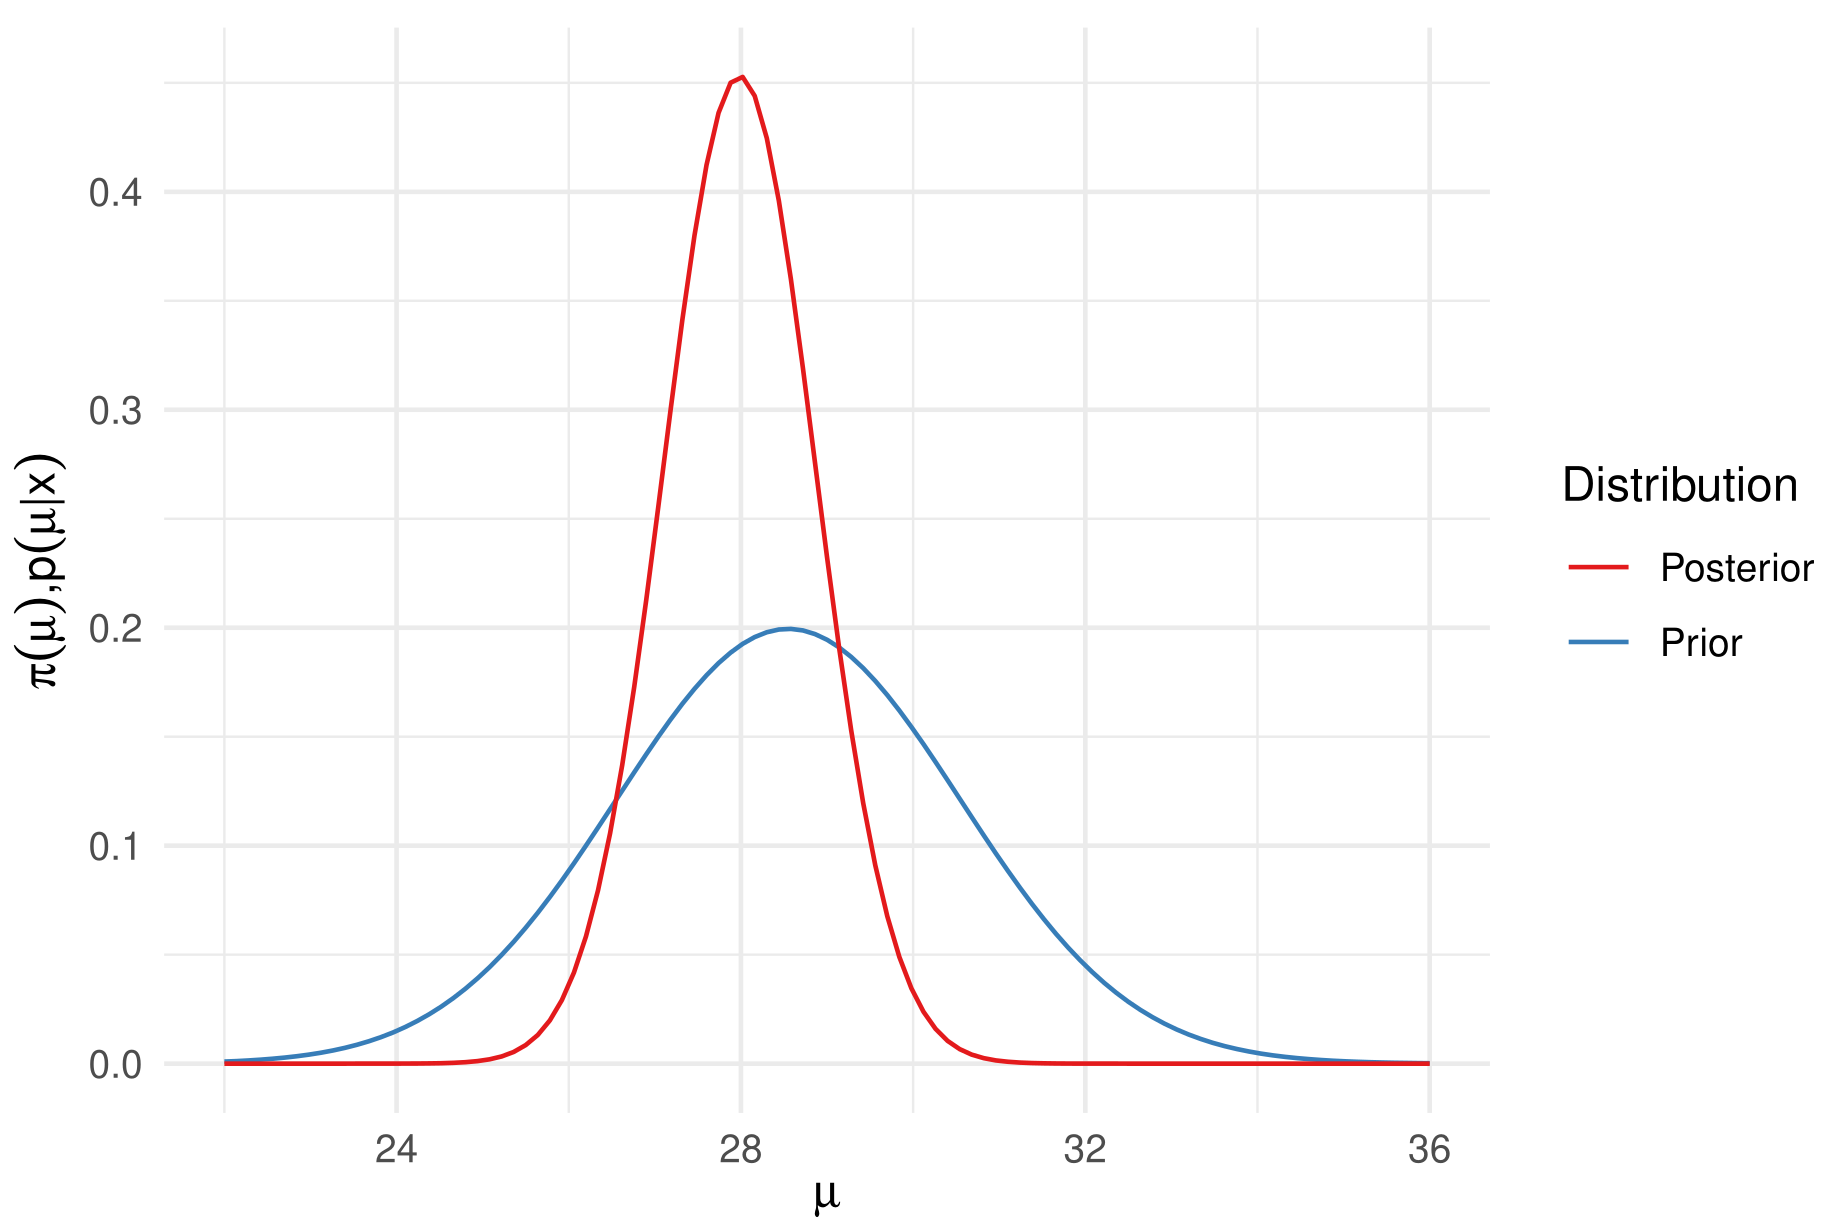
\includegraphics[width=0.7\textwidth]{img/ch2_bayes_newcomb.png}
    \caption{Prior and posterior distributions for the mean deviation $\mu$ based on Newcomb's third dataset.}
    \label{fig:bayes_newcomb}
\end{figure}

\begin{minted}{R}
ggplot(data.frame(x = c(22, 36)), aes(x)) +
  geom_function(fun = dnorm,
                args = list(mean = mu0, sd = tau),
                aes(colour = "Prior")) +
  geom_function(fun = dnorm,
                args = list(mean = post_mean, sd = post_sd),
                aes(colour = "Posterior")) +
  scale_color_brewer(palette = "Set1") +
  labs(colour = "Distribution",
       x = expression(mu),
       y = expression(paste(pi(mu), ", ", p(mu * "|" * x))))
\end{minted}

This example illustrates a key feature of Bayesian inference: information can be incorporated sequentially. 
Updating the prior using one dataset and then treating the resulting posterior as the prior for subsequent data yields the same result as combining all datasets at once, provided the observations are conditionally independent. 
The posterior distribution thus represents a complete summary of current knowledge, and any further inference—such as point estimates, credible intervals, or decision-making under loss—can be carried out directly from it.

\end{ex}

\subsubsection{Credible Intervals}
\label{sub:credible_intervals}
\begin{quote}
\emph{Given the data and the prior assumptions, which values of $\mu$ are most plausible?}
\end{quote}

In the Bayesian framework, interval estimates are obtained by identifying regions of the parameter space that carry a prescribed amount of posterior probability. Such intervals are called \textbf{credible intervals}.

For the posterior distribution of the mean deviation $\mu$ obtained in the Newcomb example, which is normal with mean $\texttt{post\_mean}$ and standard deviation $\texttt{post\_sd}$, a $95\%$ credible interval can be computed directly from the posterior quantiles:
\begin{minted}{R}
qnorm(c(0.025, 0.975), mean = post_mean, sd = post_sd)
# [1] 26.25691 29.70821
\end{minted}

Thus, the interval $(26.26,\,29.71)$ contains $\mu$ with posterior probability $95\%$. 

\medskip
\noindent
In contrast to confidence intervals, credible intervals do not rely on long-run frequency guarantees over repeated samples. 
Instead, they summarize uncertainty about $\mu$ directly through the posterior distribution.
For this reason, credible intervals are specific to Bayesian inference and should not be confused with confidence intervals, even though in some cases their numerical values may be similar.

In the Gaussian case considered here, the posterior density is symmetric and unimodal. 
A natural choice of credible interval is therefore obtained by trimming $2.5\%$ of the posterior probability mass from each tail, yielding the central $95\%$ interval. 
Equivalently, this corresponds to selecting the $2.5$th and $97.5$th percentiles of the posterior distribution.
For more general or skewed posterior distributions, one may instead consider highest posterior density (HPD) regions, which give the shortest interval containing a specified posterior probability.

\medskip
\noindent
In simple models such as the Gaussian–Gaussian setting, the posterior distribution can be derived in closed form, and posterior summaries such as means, variances, or credible intervals are easy to compute analytically.
However, for more complex likelihood–prior combinations, the posterior density may not have a tractable normalization constant or an explicit formula.

In such cases, direct analytical calculation is replaced by simulation.
If we are able to generate samples from the posterior distribution, then posterior expectations, quantiles, and credible intervals can be approximated numerically using Monte Carlo averages.
This observation motivates the use of \emph{Markov Chain Monte Carlo (MCMC)} methods, which allow us to sample from the posterior distribution whenever we can evaluate a function proportional to it.
But \emph{remember}, Bayesian computation relies on the identity
\[
\text{posterior} \;\propto\; \text{likelihood} \times \text{prior}.
\]

\medskip
\noindent
Once the posterior distribution is available—either analytically or via simulation—it represents a complete summary of current knowledge about the parameter.
Point estimates (such as posterior means or medians), interval estimates (credible intervals), and decision-theoretic procedures can all be derived from it in a unified and coherent way.

%\myparagraph{Some comments:}%
%\label{par:Some comments:}
%\begin{itemize}[]
%    \item For more general models (or rather, model--prior pairs), we may not be able to compute the posterior in closed form. 
%        But we are often able to sample from the posterior an use these samples to approximate characteristics of interest.
%        \item This is where Markov Chain Monte Carlo (MCMC) algorithms come in. They allow us to sample from the posterior provided we can evaluate a function that is proportional to the posterior density.
%            But \textit{remember}: `posterior \(\propto  \) likelihood \(\times \) prior'!
%\end{itemize}

\section{Mean Square Error, Bias and Variance}%
\label{sec:mse}
Define 
\[
    \text{MSE}_{\theta}[\hat{\theta}] :=
    \mathsf{E}_{\theta}[(\hat{\theta}-\theta)^2] = \int_{\cc{X}}^{} (\theta(x)-\theta)^2 d \mathsf{P}_{\theta}(x).
\]

\begin{theo}[]
\label{theo:mse}
    The \textbf{mean square error} decomposes as 
    \[
        \text{MSE}_{\theta}[\hat{\theta}] = (\text{Bias}_{\theta}[\hat{\theta}])^2 + \mathsf{Var}_{\theta}[\hat{\theta}],
    \]
    where \(\text{Bias}_{\theta}[\hat{\theta}] := \mathsf{E}_{\theta}[\hat{\theta}] - \theta\) is the \textbf{bias} of \(\hat{\theta}\). 
\end{theo}
\begin{proof}
    Write \(\text{MSE}_{\theta}[\hat{\theta}] = \mathsf{E}_{\theta}\left[ (\hat{\theta}-\mathsf{E}_{\theta}[\hat{\theta}]+\mathsf{E}_{\theta}[\hat{\theta}]-\theta)^2 \right]\)
    and expand
    \begin{align*}
        \text{MSE}_{\theta}[\hat{\theta}]
        &= \mathsf{E}_{\theta}\left[ (\hat{\theta}-\mathsf{E}_{\theta}[\hat{\theta}])^2 \right]
           + 2\mathsf{E}_{\theta}\left[ (\hat{\theta}-\mathsf{E}_{\theta}[\hat{\theta}])(\mathsf{E}_{\theta}[\hat{\theta}]-\theta) \right]
           + \mathsf{E}_{\theta}\left[(\mathsf{E}_{\theta}[\hat{\theta}]-\theta)^2 \right]   \\
        &= \mathsf{Var}_{\theta}[\hat{\theta}] + \mathsf{E}_{\theta}\left[  (\text{Bias}_{\theta}[\hat{\theta}])^2 \right] + 2 \cdot \text{Bias}_{\theta}[\hat{\theta}] \cdot \underbrace{\mathsf{E}_{\theta}\left[ \hat{\theta}-\mathsf{E}_{\theta}[\hat{\theta}] \right]}_{=0} \\
        &= \mathsf{Var}_{\theta}[\hat{\theta}] + (\text{Bias}_{\theta}[\hat{\theta}])^2.
    \end{align*}
\end{proof}

\noindent
\myparagraph{Interpretation.}
The bias--variance decomposition shows that the mean square error arises from two distinct sources:
\begin{itemize}
    \item \emph{Bias}, which captures systematic deviation of the estimator from the true parameter, and
    \item \emph{Variance}, which quantifies the variability of the estimator across repeated samples.
\end{itemize}
An estimator with small MSE must therefore balance these two components: low bias alone is insufficient if variance is large, and conversely, low variance does not compensate for substantial systematic bias.

This trade-off is fundamental and holds universally, independent of the complexity of the estimator or the model under consideration.
In many settings, especially in high-dimensional problems or with limited data, it can be advantageous to accept a small amount of bias in order to achieve a substantial reduction in variance.

\myparagraph{Optimality with respect to mean square error}
\label{par:optimality_mse}

\emph{Question.}  
Does there exist an estimator that is optimal in the sense of minimizing the mean square error?

More precisely, for a fixed $\theta \in \Theta$, which estimator minimizes
\[
\text{MSE}_{\theta}[\hat{\theta}]?
\]

While for a fixed value of $\theta$ such an estimator can always be constructed, there exists \emph{no} estimator that minimizes $\text{MSE}_{\theta}[\hat{\theta}]$ uniformly over all $\theta \in \Theta$, provided the statistical model contains at least two distinct distributions.

\medskip
\noindent
\textbf{Explanation.}
Fix $\theta \in \Theta$.  
The constant estimator $\hat{\theta}(x) \equiv \theta$ has mean square error
\[
\text{MSE}_{\theta}[\hat{\theta}] = 0,
\]
since it has zero bias and zero variance under $\mathsf{P}_{\theta}$.
Thus, for each individual value of $\theta$, there exists an estimator that is optimal at that specific point.

Suppose, however, that there were an estimator $\hat{\theta}^\star$ that minimized $\text{MSE}_{\theta}[\hat{\theta}]$ simultaneously for all $\theta \in \Theta$.
Then $\hat{\theta}^\star$ would have to achieve zero mean square error for every $\theta$, since it must outperform all constant estimators.
In particular,
\[
\text{MSE}_{\theta}[\hat{\theta}^\star] = 0
\quad \text{for all } \theta.
\]

By the bias--variance decomposition, this implies both
\[
\mathsf{Var}_{\theta}[\hat{\theta}^\star] = 0
\quad \text{and} \quad
\text{Bias}_{\theta}[\hat{\theta}^\star] = 0
\quad \text{for all } \theta.
\]
Zero variance implies that $\hat{\theta}^\star$ is almost surely constant under every $\mathsf{P}_{\theta}$.
However, a constant estimator cannot be unbiased for more than one value of $\theta$.
This contradiction shows that a uniformly MSE-optimal estimator cannot exist.

\medskip
\noindent
\textbf{Consequences.}
Since uniform optimality with respect to mean square error is impossible, optimality theory proceeds by modifying the criterion. Common approaches include:
\begin{itemize}
    \item Restricting attention to a class of estimators with additional properties, such as unbiasedness or equivariance, and seeking optimality within that class.
    \item Summarizing the function $\theta \mapsto \text{MSE}_{\theta}[\hat{\theta}]$ by a single number, for example by averaging with respect to a probability measure on $\Theta$ (leading to Bayes risk), or by considering the worst-case value (minimax risk).
\end{itemize}

\myparagraph{Gaussian mean: sample mean versus Bayes estimator}
\label{par:gauss_vs_bayes}

Consider the Gaussian location model
\(
X_1,\dots,X_n \stackrel{\text{i.i.d.}}{\sim} \mathcal{N}(\mu,\sigma^2),
\)
where $\sigma^2>0$ is known. We compare two estimators of the unknown mean $\mu$ and study their mean square error (MSE) as a function of $\mu$.

\begin{enumerate}[]
    \item 
\emph{Sample mean:} 
$\hat{\mu}_1=\overline{X}_n$.
Since $\mathsf{E}_{\mu}[\overline{X}_n]=\mu$, the sample mean is unbiased:
\[
\text{Bias}_{\mu}[\hat{\mu}_1]=0.
\]
Its variance is $\mathsf{Var}_{\mu}[\overline{X}_n]=\sigma^2/n$, and therefore
\[
\text{MSE}_{\mu}[\hat{\mu}_1]
=\mathsf{Var}_{\mu}[\hat{\mu}_1]
=\frac{\sigma^2}{n}.
\]
The MSE of the sample mean is constant in $\mu$: it depends only on the noise level $\sigma^2$ and the sample size $n$.

\item 
\emph{Bayes estimator:}
now consider a Bayesian estimator obtained as the posterior mean under a Gaussian prior
\(
\mu \sim \mathcal{N}(m,\tau^2)
\)
with $m=0$ and $\tau^2=1$. 

The resulting Bayes estimator $\hat{\mu}_2$ is a shrinkage estimator that pulls the sample mean toward the prior mean.
A direct calculation yields
\[
\text{Bias}_{\mu}[\hat{\mu}_2]
= -\frac{\mu\,\sigma^2}{n+\sigma^2},
\qquad
\mathsf{Var}_{\mu}[\hat{\mu}_2]
= \frac{n\sigma^2}{(n+\sigma^2)^2}.
\]
Unlike the sample mean, the Bayes estimator is biased, but its variance is smaller.
Combining bias and variance gives the mean square error
\[
\text{MSE}_{\mu}[\hat{\mu}_2]
= \frac{\sigma^2(\mu^2\sigma^2+n)}{(n+\sigma^2)^2},
\]
which is a quadratic function of $\mu$.
\end{enumerate}

\noindent
\textbf{Comparison of MSE curves.}
To illustrate the bias--variance trade-off, consider $n=10$ and $\sigma^2=1$.
\autoref{fig:mse_vs_bayes} shows the MSE of both estimators as a function of $\mu$.

\begin{minted}{R}
ggplot(data.frame(x = c(-3, 3)), aes(x)) +
  geom_function(fun = function(mu) 1 / 10,
                aes(colour = "Sample mean")) +
  geom_function(fun = function(mu) (mu^2 + 10) / (10 + 1)^2,
                aes(colour = "Bayes")) +
  scale_color_brewer(palette = "Set1") +
  labs(colour = "Estimator",
       x = expression(mu),
       y = "MSE")
\end{minted}

\begin{figure}[htpb]
    \centering
    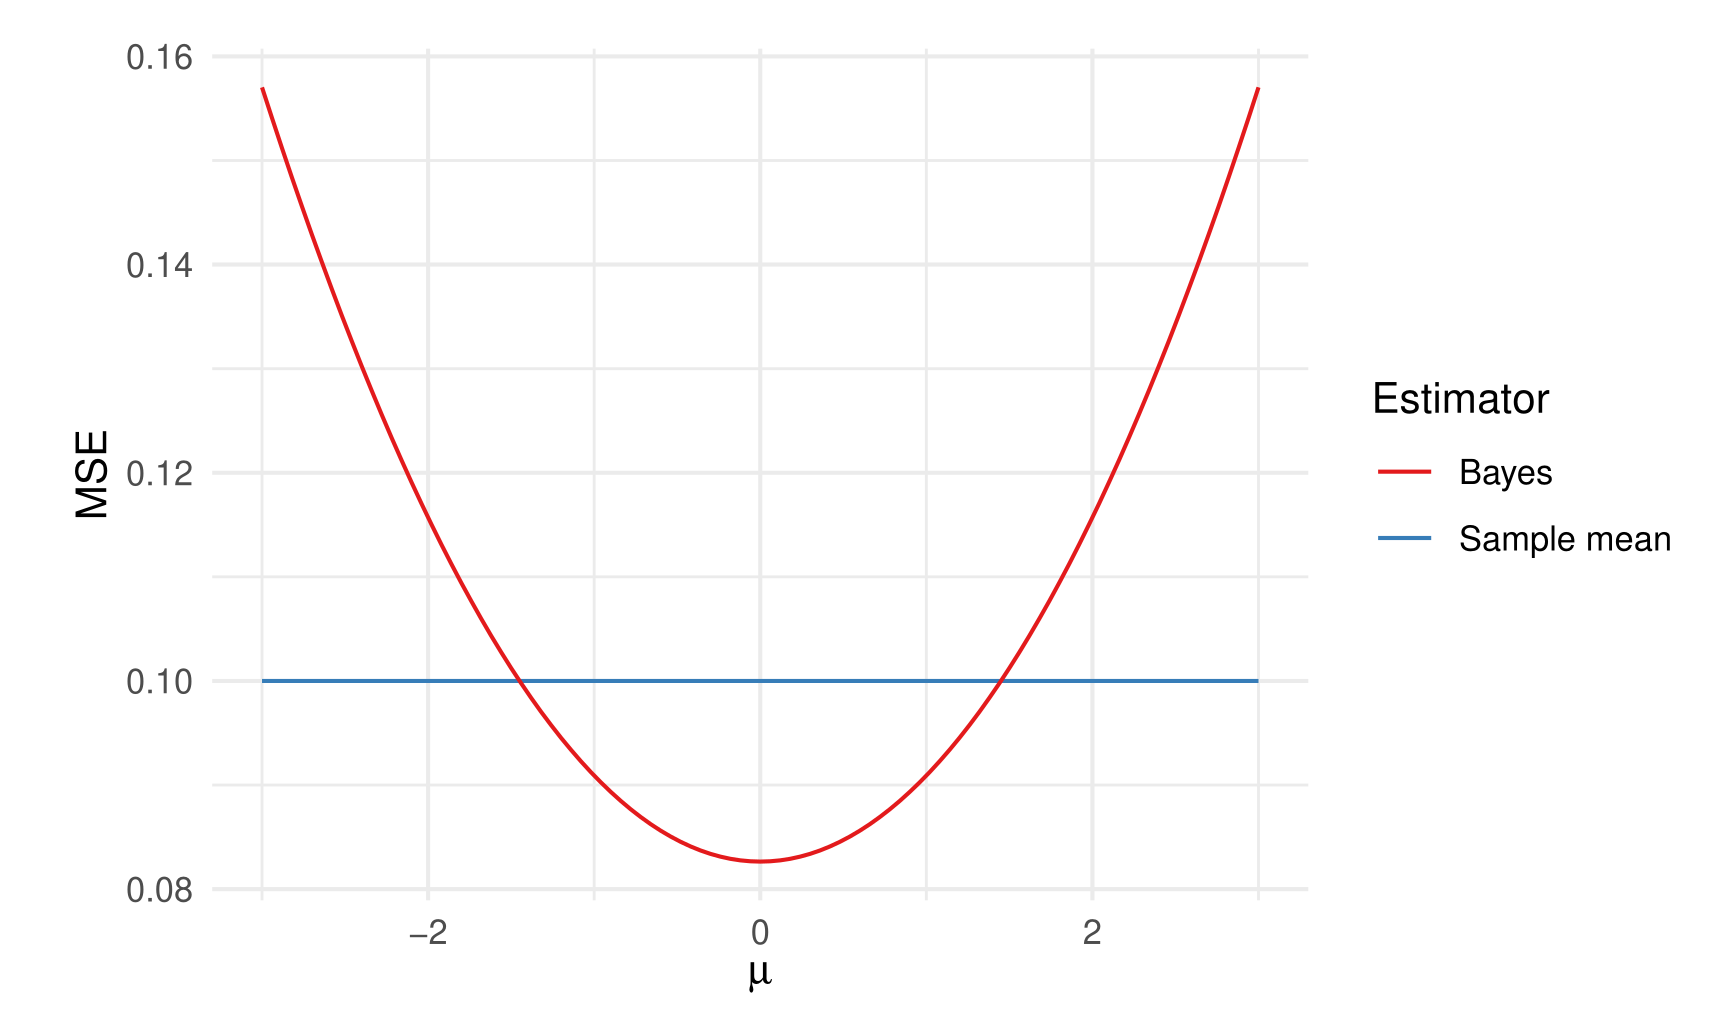
\includegraphics[width=0.8\textwidth]{img/cha2_mse_vs_bayes}
    \caption{Mean square error as a function of $\mu$ for the sample mean and a Bayes estimator with prior $\mathcal{N}(0,1)$.}
    \label{fig:mse_vs_bayes}
\end{figure}

The sample mean has constant MSE and is equally accurate for all values of $\mu$.
In contrast, the Bayes estimator performs better when $\mu$ is close to the prior mean, where the reduction in variance outweighs the introduced bias.
However, when $\mu$ is far from the prior mean, the bias dominates and the MSE increases substantially.
This example illustrates how incorporating prior information can reduce MSE locally, at the price of worse performance when the prior is badly misspecified.

\section{Discussion}
\label{sec:discussion}

\begin{itemize}
    \item \textbf{Plug--in principle.}
    \begin{itemize}
        \item A general and flexible approach for estimating complex functionals by replacing unknown distributions with their empirical counterparts.
        \item Applicable beyond simple examples, e.g.\ for measuring dependence via Hoeffding’s statistic
        \[
        D = \int \bigl(F(x,y)-F(x)F(y)\bigr)^2 \,\mathrm{d}F(x,y),
        \]
        which vanishes under independence and is positive for nonlinear dependence.
    \end{itemize}

    \item \textbf{Maximum likelihood estimation (MLE).}
    \begin{itemize}
        \item MLEs remain useful even when closed-form solutions are unavailable and numerical optimization is required.
        \item In regular models, asymptotic theory ensures optimality of the MLE for large sample sizes.
        \item Asymptotic normality allows uncertainty quantification (confidence intervals, $p$-values) using Hessian information at the optimum.
        \item This methodology underlies standard output in statistical software (e.g.\ regression models).
    \end{itemize}

    \item \textbf{Method of moments (MoM).}
    \begin{itemize}
        \item Some models admit simple, closed-form MoM estimators when MLEs are difficult or computationally expensive.
        \item Particularly useful for theoretical analysis, such as deriving lower bounds on estimation accuracy.
        \item While sometimes suboptimal, MoM estimators can provide insight and practical solutions.
    \end{itemize}

    \item \textbf{Bayesian estimation.}
    \begin{itemize}
        \item Especially valuable when data are scarce and prior information can meaningfully improve inference.
        \item Suitable priors can encode low-dimensional structure in high-dimensional problems.
        \item The Bayesian framework naturally provides uncertainty quantification through the posterior distribution.
    \end{itemize}
\end{itemize}
